\newcommand{\best}[1]{\cellcolor{CadetBlue!15}{#1}}
\newcommand{\nb}[1]{\cellcolor{pink!30}{#1}}

% Model and variant shorthand
\newcommand{\zs}{UXC\textsubscript{ZS}}
\newcommand{\ft}{UXC\textsubscript{FT}}

\newcommand{\f}[1]{#1$_{\text{F}}$}
\newcommand{\ff}[1]{#1$_{\text{FF}}$}
\newcommand{\fm}[1]{#1$_{\text{FM}}$}
\newcommand{\ffm}[1]{#1$_{\text{FFM}}$}

Title-- What Carries Architectural Signal? A Code-to-Architecture Mapping Study

Abstract--Assigning source files to reference architecture modules supports conformance checking and system understanding. Identifiers, code content, static dependencies, and directory organization inform this mapping, but their usefulness depends on how they are represented and processed. We investigate the contribution of file representations, folder and member information, and dependency neighbors, defined as files connected by static dependencies. We study ten Java, C, and C++ systems with limited labels, comparing Word2Vec, Node2Vec, and UniXcoder representations with feature-only and graph-based predictors. We vary file, member, and folder graph configurations and compare predictors with and without dependency neighbors, aggregated along the dependency direction or in both directions. Representations that encode dependencies provide strong feature-only baselines, while folder nodes yield the largest and most consistent gains among graph configurations. However, these gains largely reflect information available through a directory rule and do not consistently improve predictions for files that depart from it. With file representations held fixed, dependency neighbors raise the median score of a multilayer perceptron (MLP) receiving each file's representation and the mean representation of its neighbors, of a Graph Attention Network (GAT), and of a Heterogeneous Graph Transformer (HGT) when aggregated in both directions, with the smallest gain for HGT. Aggregating only along the dependency direction lowers median macro-F1 with Node2Vec, and the better direction depends on the system and not on the predictor or the representation. Useful dependency information therefore does not by itself determine whether neighbor aggregation helps. Evaluations should distinguish information already encoded in file representations from the contribution of neighbor access and its direction, and assess directory-departing files separately from aggregate performance.

% ___________ a_introduction _____________
\section{Introduction\label{sec:intro}}

Maintaining a software architecture requires knowing which implementation elements belong to its modules. That correspondence can become difficult to maintain as a system grows: new files introduce responsibilities and dependencies, while architectural documentation may lag behind the implementation. Code-to-architecture (C2A) mapping addresses this problem by assigning source files to the modules of a reference architecture. The resulting mapping supports reflexion modeling, which compares implementation dependencies with architectural relations to identify divergence~\cite{reflexion1}. It therefore connects the modular decomposition used to reason about a system~\cite{parnas1972,clements2003} to the code in which that decomposition is realized.
 
Several sources of evidence can support a mapping. Identifiers express domain concepts and implementation roles. Contextual code representations capture information from declarations and operations. Static dependencies locate a file among other files with which it interacts, while directories record how developers organize the project~\cite{sarif,negar,garcia2013}. These sources need not agree: a utility may depend on several modules, terminology may be shared across responsibilities, and a directory may contain files assigned to different architectural modules.
 
The usefulness of an information source also depends on how it enters a predictor. A dependency embedding can encode graph structure before a classifier sees a file. Propagating over dependencies then supplies a second form of access to related files, with its own assumptions about direction, relation types, and aggregation. A gain from the embedding does not establish that this additional propagation will help. Similarly, a folder-aware model can improve overall agreement with a reference architecture while losing correct predictions for files that depart from a directory-based assignment. These distinctions motivate studying both the information supplied to a model and the changes caused by the way it processes that information.

Prior architecture recovery and mapping work provides several ways to represent these sources. NEGAR learns structural representations using Node2Vec random walks on the dependency graph~\cite{negar}; GAER used a graph autoencoder with Word2Vec identifier embeddings for recovery~\cite{gaer}; prior mapping work uses lexical and organizational features with graph convolutional networks~\cite{jabeen2025graph}. Later work compares random walk-based methods with graph attention and diffusion-based rewiring and examines alternative uses of dependencies and folders~\cite{structsar}. These studies generally fix the representation chosen for each source, so it remains unclear which signal provides the strongest architectural evidence and how it should be represented.

We study this question through C2A mapping, a prerequisite for reflexion modeling~\cite{reflexion1}. We formulate C2A mapping as a classification problem in which each file is assigned to one module of the reference architecture. We work in a low-label setting, where about 5\% of the files are already mapped, and the model infers the remaining assignments. The model is trained on the labeled files alone. This setting allows us to examine how file representations and graph relations contribute under limited supervision.

Our evaluation uses ten Java, C, and C++ systems and covers lexical Word2Vec, structural Node2Vec, and contextual UniXcoder representations. These serve as inputs to a graph-free neural baseline, to a Heterogeneous Graph Transformer (HGT)~\cite{hgt}, and, in the dependency comparison, to a neighbor MLP and a Graph Attention Network (GAT)~\cite{gat}. The heterogeneous configurations contain file nodes and, where applicable, folder nodes and one aggregate member node per file. They vary both the context available to a file and where feature content is stored. We compare these file representations and complement the configuration comparisons with controlled comparisons that change one design choice while holding the features, labeled splits, initialization, and training budgets fixed within each comparison.

The configuration results motivate two complementary analyses. A directory analysis distinguishes errors corrected by a model from previously correct predictions that it makes incorrect. A dependency analysis compares ways of using dependency neighbors on all ten systems, switching neighbors on and off and aggregating them along the dependency direction or in both directions.

We address three research questions:
\begin{itemize}
    \item \textbf{RQ1.} How does mapping performance vary across lexical, structural and contextual file representations?
    \item \textbf{RQ2.} How does mapping performance change when file dependencies, member nodes, and folder nodes are added to each representation?
    \item \textbf{RQ3.} How do the predictor and dependency direction affect the benefit of neighbors?
\end{itemize}

The results show that dependency information supports C2A mapping through both file representations and neighbor context, but the benefit of neighbor context depends on how it is processed. Folder organization yields the largest gains, largely reflecting information already available through a directory rule. Aggregate improvements can conceal regressions on individual files. These findings clarify how input signals and their use by a predictor affect C2A mapping across the nine systems studied\footnote{\label{fn:code}Code and data are available at \url{https://github.com/sse-lnu/hetmap}.}.
% _________ 1b_related_work _____________
\section{Related Work\label{sec:work}}

Architecture recovery and code-to-architecture mapping both infer a system's modular structure from implementation artifacts, relying on evidence that includes static dependencies, code semantics, and directory organization, among other sources. Recovery produces a decomposition without a reference architecture, while mapping assigns entities to the modules of a given one. We evaluate C2A mapping, and draw on recovery research for representations of dependencies, lexical content and project organization. We organize this work by information source while keeping the two evaluation tasks distinct.

Architecture recovery techniques have historically been built around one dominant signal. Dependency-based methods treat the system as a graph and partition it to maximize modularization quality, using search-based optimization~\cite{bunch,bunch_sahc_nahc,dagc,wca,mca_eca} or clustering over dependency-derived similarity~\cite{cct,hcc_2019,limbo,fca,neighborhood_tree_2019,gma_2021}. These perform well when dependencies align with architectural boundaries, but recovery quality is sensitive to how the graph is constructed and how relations are weighted, since shared utilities and layered interactions introduce cross-module edges. Semantic methods instead cluster artifacts by identifiers and comments in a latent space learned from source code~\cite{arc,zbr,risi2012fold} or from lexical cues~\cite{kargar2017semantic}, and directory-based methods use file names and paths as an architectural signal~\cite{file_clustering}. Non-structural signals can be noisy in isolation because reused terminology and utility directories mix entities from many modules. Hybrid methods therefore combine sources through weighted similarity fusion and many-objective remodularization~\cite{sc_misra,escrc,nsga3,sadat2019multi}, consensus clustering~\cite{ensemble_recovery}, semantic-guided propagation~\cite{evol}, or weighted graphs with community detection~\cite{sade,sarif}, using different mechanisms to combine the available evidence.

Mapping shows the same pattern from a different starting point. Early work framed the assignment of unmapped entities as orphan adoption~\cite{tzerpos1997orphan}, and HuGMe introduced attraction functions to recommend mappings between entities and modules~\cite{christl2005equipping,christl2007automated}. Subsequent methods varied the signal and the learner: information-retrieval attraction based on textual similarity~\cite{bittencourt_IR}, supervised classifiers for orphan adoption~\cite{bibi2016supervised}, and a semi-supervised Naive Bayes approach combining lexical and dependency-derived information through Concrete Dependency Abstraction~\cite{olsson2019semi,olsson2022automatically}. Interactive and text-based approaches followed, comparing text classifiers for module assignment~\cite{florean2021textclassifierscomparison}, recommending mappings from natural-language architecture descriptions~\cite{InMap}, and integrating package- and class-level granularity~\cite{sinkala2023integrated}. More recent work frames method-level mapping as text classification over TF-IDF, GloVe, and LLM representations~\cite{johansson2024mapping}, examines how textual data properties condition embedding-based classification performance~\cite{johansson2025mapping}, and extracts architectural concepts from documentation and code~\cite{fuchss2025enabling}; LLM-based chain-of-thought prompting has also been used to map implementation units to a reference architecture~\cite{rukmono_deductive}, though such prompting-based approaches face scalability challenges on large codebases given context-size limits and the cost of repeatedly processing implementation artifacts.

Representation-learning approaches differ in both the information they encode and the operations used to recover or predict modules. NEGAR clusters node2vec embeddings from the dependency graph alone, with no node semantics~\cite{negar}. Jabeen et al.~\cite{structsar} build on this by adding folder organization and comparing node2vec, meta-path walks, and graph attention with and without diffusion rewiring, without lexical features. GAER and Jabeen et al.~\cite{gaer,arl_2026} instead fix folder and identifier tokens into one encoding, Word2Vec-based in the former and contrastively trained with edge attributes in the latter, without comparing it to alternatives. For mapping, prior work evaluated graph neural networks on homogeneous and dependency-type-aware graphs~\cite{jabeen2025graph}, without folder hierarchies, containment, member-level artifacts, or separating graph contribution from feature contribution. These approaches motivate our distinction between representing an information source and using it during prediction. Our configuration comparisons span lexical, structural and contextual inputs, but retain differences between their training procedures and feature content. We therefore complement them with matched dependency controls and directory-error analyses. These controls assess specific design choices; they do not turn the broader configuration comparison into an isolated ranking of information sources.

% 1c_background
\section{Background \label{sec:background}}

Software artifacts are naturally relational and multi-typed. A system contains folders, source files or classes, and finer-grained program elements such as methods and fields, connected through relations that include folder containment, file-to-member composition, and static code-level dependencies.

To preserve these distinctions, we represent each software system as a typed graph:
$$G=(V, E,\mathcal{A},\mathcal{R}),$$
where $V$ and $E$ are the sets of artifact nodes and relations between them, respectively. The mappings $\tau: V \rightarrow \mathcal{A}$ and $\phi: E \rightarrow \mathcal{R}$ assign node and relation types. In our most detailed configuration, $\mathcal{A}$ contains folder, file, and aggregate member types, while $\mathcal{R}$ distinguishes folder containment, file-to-member composition, and a single dependency relation that merges all file-level static dependencies. The file-level graph is homogeneous, and adding folder or member nodes makes it heterogeneous.

A relation's meaning depends on its type and the types of its source and target nodes in $G$. We describe an edge $e_{s,t}$ from node $s$ to node $t$ by the meta-relation $\langle \tau(s), \phi(e_{s,t}), \tau(t) \rangle$. For example, $\langle \text{folder}, \text{contains}, \text{file} \rangle$ captures project organization, whereas $\langle \text{file}, \text{depends on}, \text{file} \rangle$ captures code-level coupling. These meta-relations preserve the distinction between structural organization and implementation dependencies, which a homogeneous graph with one node type and one relation type does not explicitly represent.

HGT~\cite{hgt} exploits such meta-relations during message passing by conditioning attention and message transformation on the source node type, edge type, and target node type. GAT~\cite{gat} also uses attention-based message passing, but its standard formulation does not explicitly distinguish node or relation types. HGT can also operate on a graph with a single node type and a single relation type, although this does not make its attention mechanism equivalent to that of GAT.

The initial node features determine what information is available before message passing, while graph structure determines which nodes exchange information. Depending on how they are encoded, a file's features can capture lexical evidence from its identifiers, structural evidence from its position in the dependency graph, or contextual evidence from its code.

A lexical embedding trained on identifier tokens captures naming patterns but does not explicitly encode dependency structure or implementation syntax and behavior. A graph embedding such as Node2Vec~\cite{node2vec} instead encodes structural neighborhoods without using code content. Such embeddings have been used to capture dependency-based cohesion in architecture recovery~\cite{negar,structsar}.

Contextual representations from pretrained code encoders such as UniXcoder~\cite{unixcoder} capture the syntactic and behavioral content of an implementation that lexical features miss, but their pretraining objectives do not target architectural grouping: files with similar code can belong to different modules. Contrastive learning adapts an encoder to a chosen notion of similarity by bringing designated positive pairs closer than other in-batch examples treated as negatives, using an InfoNCE objective~\cite{infonce}. Dependency-derived positive pairs encourage embeddings to reflect dependency proximity, which need not align with reference-module membership.
% ___________ 2a_methodology ____________
\section{Methodology\label{sec:method}}

This section presents the methodology for studying how architectural signals and graph design choices affect C2A mapping. We first formulate the mapping task and then describe the graphs and the structural, lexical, and contextual features used to initialize their nodes. We then present the MLP, HGT, and GAT predictors.
 
Each research question varies one of these components and holds the others fixed. RQ1 varies the file representation, using the MLP. RQ2 varies the graph variant for each representation, using HGT because it handles the node and relation types of the heterogeneous variants. RQ3 varies the predictor, comparing the neighbor MLP with GAT and HGT, and the dependency neighbors they receive.

\subsection{Problem Formulation\label{sec:problem}}
We formulate the mapping task as node classification over a software graph $G=(V, E,\mathcal{A},\mathcal{R})$, where $\mathcal{A}$ and $\mathcal{R}$ denote the sets of node and relation types. Let $V_f \subseteq V$ be the set of file nodes, which are the targets of the mapping task. A small subset $L \subset V_f$ is labeled with known architectural module assignments $Y_L$, and the remaining file nodes $U = V_f \setminus L$ are unlabeled. The task is to learn a model:
\begin{equation}
    f_{\theta}: (G, L, Y_L) \rightarrow \hat{Y}_U,
\end{equation}
where $\theta$ denotes the learnable parameters. The model is trained on the labeled files only, but all nodes of $G$, labeled and unlabeled, are part of the graph during training.
 
Each model computes a $d$-dimensional embedding $z_i$ for every file $i \in V_f$, and the architectural module of a file is predicted from this embedding.

% _______ Graph Construction ___________
\subsection{Graph Construction\label{sec:het_graph}\label{sec:graph_variants}}
We represent the software system as a graph of software artifacts connected by folder organization, member containment, and static dependencies.

To study the individual and combined contributions of folder and member information, we construct four graph variants that differ in the node types they contain. They are named after these types: F (file nodes only), FF (folder and file nodes), FM (file and member nodes), and FFM (folder, file, and member nodes). All variants retain the dependency relation. F is homogeneous, with one node type and one relation type, and the other three variants are heterogeneous. Figure~\ref{fig:graph_variants_overview} provides a visual overview.
 
\begin{figure}[h]
\centering
\resizebox{0.96\linewidth}{!}{% \documentclass[tikz,border=5pt]{standalone}
% \usepackage[T1]{fontenc}
% \usepackage{lmodern}
% \usetikzlibrary{arrows.meta,shapes.geometric}

% \begin{document}
% \begin{tikzpicture}[
%   x=1cm,y=1cm,
%   font=\normalsize,
%   folder/.style={
%       rectangle,
%       draw=black!60,
%       fill=gray!10,
%       line width=.8pt,
%       minimum width=12mm,
%       minimum height=7mm,
%       inner sep=1pt,
%     font=\normalsize
%   },
%   file/.style={
%     circle,
%     draw=black!60,
%     fill=gray!10,
%     line width=.8pt,
%     minimum size=7mm,
%     inner sep=0pt,
%     font=\normalsize
%   },
%   member/.style={
%     diamond,
%     aspect=1,
%     draw=black!60,
%     fill=gray!10,
%     line width=.8pt,
%     minimum size=8mm,
%     inner sep=1pt,
%     font=\normalsize
%   },
%   edge/.style={
%     -{Stealth[length=1.6mm,width=1.2mm]},
%     draw=black!70,
%     line width=.6pt,
%     line cap=round,
%     line join=round,
%     shorten <=1.2pt,
%     shorten >=1.5pt
%   },
%   relation/.style={
%     edge,
%     dash pattern=on 2pt off 1.5pt
%   },
%   dependency/.style={edge}
% ]

% % F: file-only graph.
% \begin{scope}[xshift=0cm]
%   \node at (.8,2.35) {\normalsize F};

%   \node[file] (f1) at (0,0) {$f_1$};
%   \node[file] (f2) at (1.6,0) {$f_2$};

%   \draw[dependency] (f1) -- (f2);
% \end{scope}

% % FM: file-member graph.
% \begin{scope}[xshift=3cm]
%   \node at (.8,2.35) {\normalsize FM};

%   \node[file] (fmf1) at (0,0) {$f_1$};
%   \node[file] (fmf2) at (1.6,0) {$f_2$};
%   \node[member] (fmm1) at (0,-1.4) {$m_1$};
%   \node[member] (fmm2) at (1.6,-1.4) {$m_2$};

%   \draw[dependency] (fmf1) -- (fmf2);
%   \draw[dependency] (fmm1) -- (fmm2);
%   \draw[relation] (fmm1) -- (fmf1);
%   \draw[relation] (fmm2) -- (fmf2);
% \end{scope}

% % FF: folder-file graph.
% \begin{scope}[xshift=6.0cm]
%   \node at (.8,2.35) {\normalsize FF};

%   \node[folder] (ffd) at (.8,1.55) {\sffamily Folder};
%   \node[file] (fff1) at (0,0) {$f_1$};
%   \node[file] (fff2) at (1.6,0) {$f_2$};

%   \draw[relation] (ffd) -- (fff1);
%   \draw[relation] (ffd) -- (fff2);
%   \draw[dependency] (fff1) -- (fff2);
% \end{scope}

% % FFM: full graph.
% \begin{scope}[xshift=9.0cm]
%   \node at (.8,2.35) {\normalsize FFM};

%   \node[folder] (ffmd) at (.8,1.55) {\sffamily Folder};
%   \node[file] (ffmf1) at (0,0) {$f_1$};
%   \node[file] (ffmf2) at (1.6,0) {$f_2$};
%   \node[member] (ffmm1) at (0,-1.4) {$m_1$};
%   \node[member] (ffmm2) at (1.6,-1.4) {$m_2$};

%   \draw[relation] (ffmd) -- (ffmf1);
%   \draw[relation] (ffmd) -- (ffmf2);
%   \draw[dependency] (ffmf1) -- (ffmf2);
%   \draw[dependency] (ffmm1) -- (ffmm2);
%   \draw[relation] (ffmm1) -- (ffmf1);
%   \draw[relation] (ffmm2) -- (ffmf2);
% \end{scope}

% \end{tikzpicture}
% \end{document}

%%%%%%%%%%%%%%%%%%%%%%%%%%%%%%%%%%%%%%%%%%%%%%%%%%%%%%%%%%%%%%%%%%%
\documentclass[tikz,border=0pt]{standalone}
\usepackage[T1]{fontenc}
\usepackage{lmodern}
\usetikzlibrary{arrows.meta,shapes.geometric}

\begin{document}

\begin{tikzpicture}[
  x=1cm,y=1cm,
  font=\sffamily\normalsize, %\fontsize{9}{11}\selectfont,
  folder/.style={
    rectangle,
    draw=black!70,
    fill=gray!10,
    line width=.75pt,
    minimum width=5mm,
    minimum height=3.5mm,
    inner sep=0pt
  },
  file/.style={
    circle,
    draw=black!70,
    fill=gray!10,
    line width=.75pt,
    minimum size=6mm,
    inner sep=0pt
  },
  member/.style={
    diamond,
    aspect=1,
    draw=black!70,
    fill=gray!10,
    line width=.75pt,
    minimum size=7mm,
    inner sep=.5pt
  },
  edge/.style={
    -{Stealth[length=1.7mm,width=1.2mm]},
    draw=black!85,
    line width=.7pt,
    line cap=round,
    line join=round,
    shorten <=1.2pt,
    shorten >=1.5pt
  },
  relation/.style={
    edge,
    dash pattern=on 2.5pt off 1.7pt
  },
  dependency/.style={edge},
  panel title/.style={
    font=\fontsize{10}{12}\selectfont
  },
  rel label/.style={
    font=\fontsize{9}{10}\selectfont\itshape,
    text=black,
    inner sep=1pt
  },
  legend text/.style={
    anchor=west,
    inner sep=0pt,
    align=left
  }
]

\begin{scope}
  \draw[
    draw=gray!20,
    line width=.4pt,
    rounded corners=3pt
  ] (-.15,1.05) rectangle (2.55,5.2);

  \node[folder] at (.3,4.8) {};
  \node[legend text] at (.7,4.8) {Folder};

  \node[file,minimum size=5mm] at (.3,4.05) {};
  \node[legend text] at (.7,4.05) {File};

  \node[member,minimum size=6mm] at (.3,3.3) {};
  \node[legend text] at (.7,3.3) {Member};

  \draw[relation] (0,2.4) -- (.6,2.4);
  \node[legend text] at (.7,2.4) {Structural};

  \draw[dependency] (0,1.5) -- (.6,1.5);
  \node[legend text] at (.7,1.5) {Dependency};
\end{scope}

% Graph panels.
\begin{scope}[xshift=2.8cm]

  % F: upper left.
  \begin{scope}[shift={(0,6)}]
    \node[panel title] at (1,.75) {\normalsize F};

    \node[file] (f1) at (0,0) {$f_1$};
    \node[file] (f2) at (2,0) {$f_2$};

    \draw[dependency] (f1) -- (f2);
  \end{scope}

  % FM: upper right.
  \begin{scope}[shift={(4,6)}]
    \node[panel title] at (1,.75) {\normalsize FM};

    \node[file] (fmf1) at (0,0) {$f_1$};
    \node[file] (fmf2) at (2,0) {$f_2$};
    \node[member] (fmm1) at (0,-1.3) {$m_1$};
    \node[member] (fmm2) at (2,-1.3) {$m_2$};

    \draw[dependency] (fmf1) -- (fmf2);
    \draw[dependency] (fmm1) -- (fmm2);
    \draw[relation] (fmm1) -- (fmf1);
    \draw[relation] (fmm2) -- (fmf2);
  \end{scope}

  % FF: lower left.
  \begin{scope}
    \node[panel title] at (1,3.65) {\normalsize FF};

    \node[folder] (ffp) at (1,2.9) {};
    \node[folder] (ffd) at (1,1.6) {};
    \node[file] (fff1) at (0,0) {$f_1$};
    \node[file] (fff2) at (2,0) {$f_2$};

    \draw[relation] (ffp) -- (ffd);
    \draw[relation] (ffd) -- (fff1);
    \draw[relation] (ffd) -- (fff2);
    \draw[dependency] (fff1) -- (fff2);
  \end{scope}

  % FFM: lower right, with edge labels retained.
  \begin{scope}[xshift=4cm]
    \node[panel title] at (1,3.65) {\normalsize FFM};

    \node[folder] (ffmp) at (1,2.9) {};
    \node[folder] (ffmd) at (1,1.6) {};
    \node[file] (ffmf1) at (0,0) {$f_1$};
    \node[file] (ffmf2) at (2,0) {$f_2$};
    \node[member] (ffmm1) at (0,-1.3) {$m_1$};
    \node[member] (ffmm2) at (2,-1.3) {$m_2$};

    \draw[relation] (ffmp) -- (ffmd)
      node[rel label,midway,left=3pt] {parent\_of};

    \draw[relation] (ffmd) -- (ffmf1)
      node[rel label,midway,left=3pt] {contains};

    \draw[relation] (ffmd) -- (ffmf2);

    \draw[dependency] (ffmf1) -- (ffmf2)
      node[rel label,midway,below=4pt] {depends\_on};

    \draw[dependency] (ffmm1) -- (ffmm2)
      node[rel label,midway,below=4pt] {depends\_on};

    \draw[relation] (ffmm1) -- (ffmf1)
      node[rel label,midway,left=3pt] {belongs\_to};

    \draw[relation] (ffmm2) -- (ffmf2);
  \end{scope}

\end{scope}

\end{tikzpicture}

\end{document}}
\caption{Graph variants F, FM, FF, and FFM. Files $f_i$ are the prediction targets, and each $m_i$ aggregates the members of file $f_i$. Arrows point from source to target: dashed arrows are structural relations and solid arrows are dependencies. Relation names are shown on FFM only. The panels omit further dependency edges and folder levels; Table~\ref{tab:relation_types} lists the relations with the node types they connect. Feature construction also depends on the variant, as described in Section~\ref{sec:node_features}.}
\label{fig:graph_variants_overview}
\end{figure}

\subsubsection{Nodes and Relations}
The complete graph (FFM) has three node types. File nodes represent source files and are the targets of C2A mapping. Because logical components are often implemented through namespaces or directory structures that group source code providing a particular functionality~\cite{fundamentals_sa, garcia2013}, folder nodes represent directory levels of the project, with one node per level. Each file has one summarized member node covering the methods, fields, constructors, and variables of that file. This retains member-level information while avoiding the large and sparse graphs produced by representing individual members.

Four relations connect these nodes, as listed in Table~\ref{tab:relation_types}. Three are structural and encode organization and containment, and the fourth encodes static dependencies. Folder nodes are connected through \emph{parent\_of} edges, forming chains such as \texttt{app} $\rightarrow$ \texttt{app/ui} $\rightarrow$ \texttt{app/ui/views}, and \emph{contains} edges link each folder to its files. A \emph{belongs\_to} edge links each member node to its enclosing file.

Messages along structural relations flow toward the file. Folder information passes down the hierarchy through \emph{parent\_of} and \emph{contains} edges, and member information passes up to the file through \emph{belongs\_to} edges. No reverse edges are added, so folder and member nodes are not updated from files through structural relations.

The fourth relation, \emph{depends\_on}, encodes static dependencies, which provide direct evidence of how source files interact~\cite{negar, deps_impact}. Dependencies were extracted with the Depends tool~\cite{depends}, which analyzes the syntactic structure of the projects and identifies entities together with several categories of static relations. We merge all dependency types into a single relation, drop duplicate edges, and remove edges whose endpoints belong to the same file.

Dependency endpoints depend on the graph variant. In FM and FFM, dependencies connect either two files or two member nodes. Dependencies between a file and a member are resolved between their corresponding files. In F and FF, all member endpoints are replaced by their enclosing files, so all dependencies connect file nodes.

RQ1 uses no graph structure, and RQ3 uses the homogeneous file-level graph F. RQ2 uses all four variants to examine progressively richer graph structure, adding folder nodes in FF, member nodes in FM, and both in FFM.

\begin{table}[htb]
\centering
\caption{Graph relations and node types.}
\label{tab:relation_types}
\renewcommand{\arraystretch}{1.0}
\setlength{\tabcolsep}{4pt}
\begin{tabularx}{\columnwidth}{@{}l l >{\raggedright\arraybackslash}X@{}}
\toprule
Relation & Source $\to$ target & Description \\
\midrule
\emph{parent\_of}
& folder $\to$ folder
& Directory hierarchy. \\
\emph{contains}
& folder $\to$ file
& Folder contains a file. \\
\emph{belongs\_to}
& member $\to$ file
& Links a member node to its file. \\

\multirow{2}{*}{\emph{depends\_on}}
& file $\to$ file
& File-level dependencies. \\
& member $\to$ member
& Member-level dependency in FM and FFM. \\
\bottomrule
\end{tabularx}
\end{table}
% _________ Node Feature Initialization ______________
\subsection{Node Feature Initialization \label{sec:node_features}}
Folder nodes are initialized in the same way in every setting. File and member nodes are initialized with one of the representations compared in RQ1: lexical embeddings from Word2Vec, structural embeddings from Node2Vec, or contextual embeddings from UniXcoder, used zero-shot or fine-tuned with dependencies.

Member information enters the model differently across representations. Word2Vec includes member identifiers in file vectors when member nodes are absent and places them in member nodes otherwise. UniXcoder provides member text only through member nodes, while Node2Vec assigns each member node its file's vector. Adding member nodes thus changes the placement or availability of information as well as the graph structure, so comparisons across graph variants are interpreted separately for each representation.

\subsubsection{Folder Node Features}
Folder nodes use a binary bag-of-words representation of the folder tokens along their paths, after removing common project-root tokens. For example, \texttt{app/ui/views} is represented by \texttt{app}, \texttt{ui}, and \texttt{views}. Including the tokens of its ancestors preserves each folder's hierarchical context.

\subsubsection{Word2Vec (W2V): Lexical Features\label{sec:node_w2v}}
Source code identifiers encode domain concepts and implementation roles, making them useful signals for C2A mapping~\cite{sarif}. Following Jabeen et al.~\citep{gaer}, we extract tokens from file names and from the identifiers of members, namely methods, fields, constructors, and variables. We split camelCase, PascalCase, and snake\_case identifiers, convert tokens to lowercase, and remove stopwords and non-alphabetic tokens. Each node vector is the mean of the skip-gram Word2Vec embeddings of its associated tokens~\cite{word2vec}.

In FM and FFM, file nodes use file-name tokens, while member nodes use member identifiers. In F and FF, member identifiers are included in the file vector instead, and the MLP uses this same file vector. Member identifiers therefore remain available in every variant.

\subsubsection{Node2Vec (N2V): Structural Features \label{sec:node_n2v}}
Chen et al.~\citep{negar} observe that files in the same architectural module can occupy a dense local dependency region without being directly connected. They use random-walk embeddings to capture this longer-range structure for architecture recovery. In our earlier study of dependency-only recovery, which follows their setup, Node2Vec was among the best-performing learned representations~\cite{structsar}. Therefore, we use Node2Vec~\cite{node2vec} embeddings computed with uniform random walks on the undirected file-level dependency graph as a structural initialization. These embeddings encode dependency structure without using identifiers or folder location.

In FM and FFM, each summarized member node receives the Node2Vec embedding of its corresponding file.
 
\subsubsection{UniXcoder: Contextual Features \label{sec:unixcoder}}
For contextual initialization, we use UniXcoder~\cite{unixcoder}, a pretrained code transformer. We parse each source file with Tree-sitter~\cite{tree_sitter} using the corresponding Java, C, or C++ grammar. The syntax tree determines which source fragments are passed to the encoder, but is not itself an input to the model. Extraction produces two views. The file-level view contains type declarations, fields or global variables, and constructor signatures with short body excerpts where applicable. The member-level view contains methods or functions. Each view produces one vector per file. Member-level text is split into overlapping chunks whose embeddings are mean-pooled.
 
The zero-shot variant (\zs{}) uses the pretrained weights. The dependency-guided variant (\ft{}) is fine-tuned separately for each system with a contrastive objective~\cite{infonce} using dependency-based positive pairs. Fine-tuning uses only the file-level views, and module labels do not enter the loss. The fine-tuned encoder then encodes both views and produces one vector per view for each file, so member-level text is encoded but is not part of the fine-tuning objective.
 
Positive pairs are drawn from the two-hop neighborhood to capture longer-range dependency structure~\cite{structsar}, with dependencies treated as undirected. For each anchor file, two positives are sampled at random from the eight two-hop candidates that share the most one-hop neighbors with it. Files without a two-hop candidate fall back to a direct neighbor. Other files in the batch serve as negatives, except directly connected files, which are masked unless selected as the positive pair.
% __________ Model ________________
\subsection{Mapping Models\label{sec:mapping_models}}
We compare models that use file features alone with models that incorporate graph structure. RQ1 uses the MLP, RQ2 uses HGT, and RQ3 compares the neighbor MLP, GAT, and HGT. All models use the same classification head to predict architectural modules. Throughout, $\mathcal{N}(\cdot)$ denotes the neighborhood of a node.

\subsubsection{Multilayer Perceptron (MLP)\label{sec:mlp}}
The MLP predicts module logits directly from a file-level input vector. Each hidden layer computes:
\begin{equation}
h_i^{(k+1)} = \text{ReLU}\big(W^{(k)} h_i^{(k)} + b^{(k)}\big),
\end{equation}
with $h_i^{(0)} = x_i$ the file feature vector and $W^{(k)}, b^{(k)}$ the learnable parameters of layer $k$, and ReLU is the rectified linear unit~\cite{relu}. The input $x_i$ contains the single representation being evaluated.
 
For RQ3, we incorporate dependency neighborhood information in the MLP by concatenating each file's vector $x_i$ with the mean $\bar{x}_{\mathcal{N}(i)}$ of its direct neighbors' vectors in the dependency graph, giving $[x_i \,\|\, \bar{x}_{\mathcal{N}(i)}]$. We refer to the MLP with this input as the neighbor MLP (\mlp{}).
 
\subsubsection{Heterogeneous Graph Transformer (HGT)\label{sec:hgt_model}}
Node types have different feature spaces depending on the graph variant and the initialization strategy, so HGT first maps the input vector $x_t$ of each node $t$ into a shared hidden space using a type-specific linear transformation followed by ReLU, which gives its initial representation $h_t^{(0)}$. One HGT layer~\cite{hgt} then updates node representations through multi-head attention over their neighbors.
 
For a target node $t$ and a source node $s$ connected by an edge $e$, the layer computes a message $M(s,e,t)$ and an attention weight $\alpha(s,e,t)$, and aggregates them as:
\begin{align}
m_t &= \sum_{s \in \mathcal{N}(t)} \alpha(s,e,t)\, M(s,e,t), \\
M(s,e,t) &= W^{\mathrm{MSG}}_{\phi(e)}\, V_{\tau(s)}\, h_s, \notag \\
\alpha(s,e,t) &= \operatorname*{softmax}_{s \in \mathcal{N}(t)} \frac{\big(K_{\tau(s)} h_s\big)^{\top} W^{\mathrm{ATT}}_{\phi(e)}\, \big(Q_{\tau(t)} h_t\big)\, \mu_{\langle \tau(s),\phi(e),\tau(t)\rangle}}{\sqrt{d_h}}. \notag
\end{align}
\noindent where $\tau(\cdot)$ is the node type, $\phi(e)$ is the edge type, $V$, $K$, and $Q$ are type-specific linear transformations, $W^{\mathrm{MSG}}$ and $W^{\mathrm{ATT}}$ are edge-type-specific matrices, $\mu$ is a learned prior for each meta-relation, $d_h$ is the head dimension, and attention-head indices are omitted for brevity. These parameters allow a \emph{contains} edge from a folder and a \emph{depends\_on} edge from a dependent file to receive different attention weights.
 
Finally, the aggregated message is combined with the node's projected input $h_t^{(0)}$ through a residual connection~\cite{residual_connection} followed by layer normalization:
\begin{equation}
h_t^{(1)} = \mathrm{LayerNorm}\left(m_t + h_t^{(0)}\right).
\end{equation}
Folder and member nodes, when present, contribute to file representations through message passing.
 
\subsubsection{Graph Attention Network (GAT)\label{sec:gat_model}}
GAT~\cite{gat} aggregates neighbor representations using attention parameters shared across neighbors within each head, without the node-type- or edge-type-specific parameters of HGT. The outputs of the attention heads are concatenated. Our GAT implementation uses the same input projection, residual connection, and layer normalization as HGT, while replacing its neighbor aggregation mechanism. We add no self-loops; the residual connection retains the node's own representation.
 
\subsubsection{Classification Head\label{sec:head}}
All three predictors use the same classification head. The file embedding $z_i \in \mathbb{R}^{d}$, obtained from the last hidden layer of the MLP or the message-passing layer of GAT and HGT, is passed to a linear layer that produces one score per architectural module. A softmax converts these scores into a probability distribution:
\begin{equation}
\label{eq:head}
\begin{aligned}
p_i &= \text{softmax}\big(W_c z_i + b_c\big), \\
\hat{y}_i &= \arg\max_m p_{i,m},
\end{aligned}
\end{equation}
where $W_c \in \mathbb{R}^{|M| \times d}$, $b_c \in \mathbb{R}^{|M|}$, and $|M|$ is the number of architectural modules. The predicted module $\hat{y}_i$ is the one with the highest probability. Training minimizes categorical cross-entropy over the labeled file nodes.
 % _______ Graph Construction ___________
\section{Methodology\label{sec:method}}

This section presents the methodology for studying how architectural signals and graph design choices affect C2A mapping. We first formulate the mapping task and then describe the graphs and the structural, lexical, and contextual features used to initialize their nodes. We then present the MLP, HGT, and GAT predictors and the dependency neighbor settings.
 
Each research question varies one of these components and holds the others fixed. RQ1 varies the file representation, using the MLP. RQ2 varies the graph variant for each representation, using HGT. RQ3 varies the predictor, comparing the neighbor MLP with GAT and HGT, and the dependency neighbors they receive.

\subsection{Problem Formulation\label{sec:problem}}
We formulate the mapping task as node classification over a software graph $G=(V, E,\mathcal{A},\mathcal{R})$, where $\mathcal{A}$ and $\mathcal{R}$ denote the sets of node and relation types. Let $V_f \subseteq V$ be the set of file nodes, which are the targets of the mapping task. A small subset $L \subset V_f$ is labeled with known architectural module assignments $Y_L$, and the remaining file nodes $U = V_f \setminus L$ are unlabeled. The task is to learn a model:
\begin{equation}
    f_{\theta}: (G, L, Y_L) \rightarrow \hat{Y}_U,
\end{equation}
where $\theta$ denotes the learnable parameters. The model is trained on the labeled files only, but all nodes of $G$, labeled and unlabeled, are part of the graph during training.
 
Each model computes a $d$-dimensional embedding $z_i$ for every file $i \in V_f$, and the architectural module of a file is predicted from this embedding.

% _______ Graph Construction ___________
\subsection{Graph Construction\label{sec:het_graph}\label{sec:graph_variants}}
We represent the software system as a graph of software artifacts connected by folder organization, member containment, and static dependencies.

To study the individual and combined contributions of folder and member information, we construct four graph variants that differ in the node types they contain. They are named after these types: F (file nodes only), FF (folder and file nodes), FM (file and member nodes), and FFM (folder, file, and member nodes). All variants retain the dependency relation. F is homogeneous, with one node type and one relation type, and the other three variants are heterogeneous. Figure~\ref{fig:graph_variants_overview} provides a visual overview.
 
\begin{figure}[h]
\centering
\resizebox{0.98\linewidth}{!}{% \documentclass[tikz,border=5pt]{standalone}
% \usepackage[T1]{fontenc}
% \usepackage{lmodern}
% \usetikzlibrary{arrows.meta,shapes.geometric}

% \begin{document}
% \begin{tikzpicture}[
%   x=1cm,y=1cm,
%   font=\normalsize,
%   folder/.style={
%       rectangle,
%       draw=black!60,
%       fill=gray!10,
%       line width=.8pt,
%       minimum width=12mm,
%       minimum height=7mm,
%       inner sep=1pt,
%     font=\normalsize
%   },
%   file/.style={
%     circle,
%     draw=black!60,
%     fill=gray!10,
%     line width=.8pt,
%     minimum size=7mm,
%     inner sep=0pt,
%     font=\normalsize
%   },
%   member/.style={
%     diamond,
%     aspect=1,
%     draw=black!60,
%     fill=gray!10,
%     line width=.8pt,
%     minimum size=8mm,
%     inner sep=1pt,
%     font=\normalsize
%   },
%   edge/.style={
%     -{Stealth[length=1.6mm,width=1.2mm]},
%     draw=black!70,
%     line width=.6pt,
%     line cap=round,
%     line join=round,
%     shorten <=1.2pt,
%     shorten >=1.5pt
%   },
%   relation/.style={
%     edge,
%     dash pattern=on 2pt off 1.5pt
%   },
%   dependency/.style={edge}
% ]

% % F: file-only graph.
% \begin{scope}[xshift=0cm]
%   \node at (.8,2.35) {\normalsize F};

%   \node[file] (f1) at (0,0) {$f_1$};
%   \node[file] (f2) at (1.6,0) {$f_2$};

%   \draw[dependency] (f1) -- (f2);
% \end{scope}

% % FM: file-member graph.
% \begin{scope}[xshift=3cm]
%   \node at (.8,2.35) {\normalsize FM};

%   \node[file] (fmf1) at (0,0) {$f_1$};
%   \node[file] (fmf2) at (1.6,0) {$f_2$};
%   \node[member] (fmm1) at (0,-1.4) {$m_1$};
%   \node[member] (fmm2) at (1.6,-1.4) {$m_2$};

%   \draw[dependency] (fmf1) -- (fmf2);
%   \draw[dependency] (fmm1) -- (fmm2);
%   \draw[relation] (fmm1) -- (fmf1);
%   \draw[relation] (fmm2) -- (fmf2);
% \end{scope}

% % FF: folder-file graph.
% \begin{scope}[xshift=6.0cm]
%   \node at (.8,2.35) {\normalsize FF};

%   \node[folder] (ffd) at (.8,1.55) {\sffamily Folder};
%   \node[file] (fff1) at (0,0) {$f_1$};
%   \node[file] (fff2) at (1.6,0) {$f_2$};

%   \draw[relation] (ffd) -- (fff1);
%   \draw[relation] (ffd) -- (fff2);
%   \draw[dependency] (fff1) -- (fff2);
% \end{scope}

% % FFM: full graph.
% \begin{scope}[xshift=9.0cm]
%   \node at (.8,2.35) {\normalsize FFM};

%   \node[folder] (ffmd) at (.8,1.55) {\sffamily Folder};
%   \node[file] (ffmf1) at (0,0) {$f_1$};
%   \node[file] (ffmf2) at (1.6,0) {$f_2$};
%   \node[member] (ffmm1) at (0,-1.4) {$m_1$};
%   \node[member] (ffmm2) at (1.6,-1.4) {$m_2$};

%   \draw[relation] (ffmd) -- (ffmf1);
%   \draw[relation] (ffmd) -- (ffmf2);
%   \draw[dependency] (ffmf1) -- (ffmf2);
%   \draw[dependency] (ffmm1) -- (ffmm2);
%   \draw[relation] (ffmm1) -- (ffmf1);
%   \draw[relation] (ffmm2) -- (ffmf2);
% \end{scope}

% \end{tikzpicture}
% \end{document}

%%%%%%%%%%%%%%%%%%%%%%%%%%%%%%%%%%%%%%%%%%%%%%%%%%%%%%%%%%%%%%%%%%%
\documentclass[tikz,border=0pt]{standalone}
\usepackage[T1]{fontenc}
\usepackage{lmodern}
\usetikzlibrary{arrows.meta,shapes.geometric}

\begin{document}

\begin{tikzpicture}[
  x=1cm,y=1cm,
  font=\sffamily\normalsize, %\fontsize{9}{11}\selectfont,
  folder/.style={
    rectangle,
    draw=black!70,
    fill=gray!10,
    line width=.75pt,
    minimum width=5mm,
    minimum height=3.5mm,
    inner sep=0pt
  },
  file/.style={
    circle,
    draw=black!70,
    fill=gray!10,
    line width=.75pt,
    minimum size=6mm,
    inner sep=0pt
  },
  member/.style={
    diamond,
    aspect=1,
    draw=black!70,
    fill=gray!10,
    line width=.75pt,
    minimum size=7mm,
    inner sep=.5pt
  },
  edge/.style={
    -{Stealth[length=1.7mm,width=1.2mm]},
    draw=black!85,
    line width=.7pt,
    line cap=round,
    line join=round,
    shorten <=1.2pt,
    shorten >=1.5pt
  },
  relation/.style={
    edge,
    dash pattern=on 2.5pt off 1.7pt
  },
  dependency/.style={edge},
  panel title/.style={
    font=\fontsize{10}{12}\selectfont
  },
  rel label/.style={
    font=\fontsize{9}{10}\selectfont\itshape,
    text=black,
    inner sep=1pt
  },
  legend text/.style={
    anchor=west,
    inner sep=0pt,
    align=left
  }
]

\begin{scope}
  \draw[
    draw=gray!20,
    line width=.4pt,
    rounded corners=3pt
  ] (-.15,1.05) rectangle (2.55,5.2);

  \node[folder] at (.3,4.8) {};
  \node[legend text] at (.7,4.8) {Folder};

  \node[file,minimum size=5mm] at (.3,4.05) {};
  \node[legend text] at (.7,4.05) {File};

  \node[member,minimum size=6mm] at (.3,3.3) {};
  \node[legend text] at (.7,3.3) {Member};

  \draw[relation] (0,2.4) -- (.6,2.4);
  \node[legend text] at (.7,2.4) {Structural};

  \draw[dependency] (0,1.5) -- (.6,1.5);
  \node[legend text] at (.7,1.5) {Dependency};
\end{scope}

% Graph panels.
\begin{scope}[xshift=2.8cm]

  % F: upper left.
  \begin{scope}[shift={(0,6)}]
    \node[panel title] at (1,.75) {\normalsize F};

    \node[file] (f1) at (0,0) {$f_1$};
    \node[file] (f2) at (2,0) {$f_2$};

    \draw[dependency] (f1) -- (f2);
  \end{scope}

  % FM: upper right.
  \begin{scope}[shift={(4,6)}]
    \node[panel title] at (1,.75) {\normalsize FM};

    \node[file] (fmf1) at (0,0) {$f_1$};
    \node[file] (fmf2) at (2,0) {$f_2$};
    \node[member] (fmm1) at (0,-1.3) {$m_1$};
    \node[member] (fmm2) at (2,-1.3) {$m_2$};

    \draw[dependency] (fmf1) -- (fmf2);
    \draw[dependency] (fmm1) -- (fmm2);
    \draw[relation] (fmm1) -- (fmf1);
    \draw[relation] (fmm2) -- (fmf2);
  \end{scope}

  % FF: lower left.
  \begin{scope}
    \node[panel title] at (1,3.65) {\normalsize FF};

    \node[folder] (ffp) at (1,2.9) {};
    \node[folder] (ffd) at (1,1.6) {};
    \node[file] (fff1) at (0,0) {$f_1$};
    \node[file] (fff2) at (2,0) {$f_2$};

    \draw[relation] (ffp) -- (ffd);
    \draw[relation] (ffd) -- (fff1);
    \draw[relation] (ffd) -- (fff2);
    \draw[dependency] (fff1) -- (fff2);
  \end{scope}

  % FFM: lower right, with edge labels retained.
  \begin{scope}[xshift=4cm]
    \node[panel title] at (1,3.65) {\normalsize FFM};

    \node[folder] (ffmp) at (1,2.9) {};
    \node[folder] (ffmd) at (1,1.6) {};
    \node[file] (ffmf1) at (0,0) {$f_1$};
    \node[file] (ffmf2) at (2,0) {$f_2$};
    \node[member] (ffmm1) at (0,-1.3) {$m_1$};
    \node[member] (ffmm2) at (2,-1.3) {$m_2$};

    \draw[relation] (ffmp) -- (ffmd)
      node[rel label,midway,left=3pt] {parent\_of};

    \draw[relation] (ffmd) -- (ffmf1)
      node[rel label,midway,left=3pt] {contains};

    \draw[relation] (ffmd) -- (ffmf2);

    \draw[dependency] (ffmf1) -- (ffmf2)
      node[rel label,midway,below=4pt] {depends\_on};

    \draw[dependency] (ffmm1) -- (ffmm2)
      node[rel label,midway,below=4pt] {depends\_on};

    \draw[relation] (ffmm1) -- (ffmf1)
      node[rel label,midway,left=3pt] {belongs\_to};

    \draw[relation] (ffmm2) -- (ffmf2);
  \end{scope}

\end{scope}

\end{tikzpicture}

\end{document}}
\caption{Graph variants F, FM, FF, and FFM. Files $f_i$ are the prediction targets, and each $m_i$ aggregates the members of file $f_i$. Arrows point from source to target: dashed arrows are structural relations and solid arrows are dependencies. Relation names are shown on FFM only. The panels omit further dependency edges and folder levels; Table~\ref{tab:relation_types} lists the relations with the node types they connect. Feature construction also depends on the variant, as described in Section~\ref{sec:node_features}.}
\label{fig:graph_variants_overview}
\end{figure}

\subsubsection{Nodes and Relations}
The complete graph (FFM) has three node types. File nodes represent source files and are the targets of code-to-architecture mapping. Because logical components are often implemented through namespaces or directory structures that group source code providing a particular functionality~\cite{fundamentals_sa, garcia2013}, folder nodes represent directory levels of the project, with one node per level. Each file has one summarized member node covering the methods, fields, constructors, and variables of that file. This retains member-level information while avoiding the large and sparse graphs produced by representing individual members.

Four relations connect these nodes, as listed in Table~\ref{tab:relation_types}. Three are structural and encode organization and containment, and the fourth encodes static dependencies. Folder nodes are connected through \emph{parent\_of} edges, forming chains such as \texttt{app} $\rightarrow$ \texttt{app/ui} $\rightarrow$ \texttt{app/ui/views}, and \emph{contains} edges link each folder to its files. A \emph{belongs\_to} edge links each member node to its enclosing file.

Messages along structural relations flow toward the file. Folder information passes down the hierarchy through \emph{parent\_of} and \emph{contains} edges, and member information passes up to the file through \emph{belongs\_to} edges. No reverse edges are added, so folder and member nodes are not updated from files through structural relations.

The fourth relation, \emph{depends\_on}, encodes static dependencies, which provide direct evidence of how source files interact~\cite{negar, deps_impact}. Dependencies were extracted with the Depends tool~\cite{depends}, which analyzes the syntactic structure of the projects and identifies entities together with several categories of static relations. We merge all dependency types into a single relation, drop duplicate edges, and remove edges whose endpoints belong to the same file.

Dependency endpoints depend on the graph variant. In FM and FFM, dependencies connect either two files or two member nodes. Dependencies between a file and a member are resolved between their corresponding files. In F and FF, all member endpoints are replaced by their enclosing files, so all dependencies connect file nodes.

RQ1 and RQ3 use the homogeneous file-level graph F for graph-based models. RQ2 uses all four variants to examine progressively richer graph structure, adding folder nodes in FF, member nodes in FM, and both in FFM.

\begin{table}[htb]
\centering
\caption{Graph relations and node types.}
\label{tab:relation_types}
\renewcommand{\arraystretch}{1.0}
\setlength{\tabcolsep}{4pt}
\begin{tabularx}{\columnwidth}{@{}l l >{\raggedright\arraybackslash}X@{}}
\toprule
Relation & Source $\to$ target & Description \\
\midrule
\emph{parent\_of}
& folder $\to$ folder
& Directory hierarchy. \\
\emph{contains}
& folder $\to$ file
& Folder contains a file. \\
\emph{belongs\_to}
& member $\to$ file
& Links a member node to its file. \\

\multirow{2}{*}{\emph{depends\_on}}
& file $\to$ file
& File-level dependencies. \\
& member $\to$ member
& Member-level dependency in FM and FFM. \\
\bottomrule
\end{tabularx}
\end{table}
% _________ Node Feature Initialization ______________
\subsection{Node Feature Initialization \label{sec:node_features}}
Folder nodes are initialized in the same way in every setting. File and member nodes are initialized with one of the representations compared in RQ1: lexical embeddings from Word2Vec, structural embeddings from Node2Vec, or contextual embeddings from UniXcoder, used zero-shot or fine-tuned with dependencies.

Member information enters the model differently across representations. Word2Vec includes member identifiers in file vectors when member nodes are absent and places them in member nodes otherwise. UniXcoder provides member text only through member nodes, while Node2Vec assigns each member node its file's vector. Adding member nodes thus changes the placement or availability of information as well as the graph structure, so comparisons across graph variants are interpreted separately for each representation.

\subsubsection{Folder Node Features}
Folder nodes use a binary bag-of-words representation of the folder tokens along their paths, after removing common project-root tokens. For example, \texttt{app/ui/views} is represented by \texttt{app}, \texttt{ui}, and \texttt{views}. Including the tokens of its ancestors preserves each folder's hierarchical context.

\subsubsection{Word2Vec (W2V): Lexical Features\label{sec:node_w2v}}
Source code identifiers encode domain concepts and implementation roles, making them useful signals for C2A mapping~\cite{sarif}. Following Jabeen et al.~\citep{gaer}, we extract tokens from file names and member identifiers, including methods, fields, constructors, and variables. We split camelCase, PascalCase, and snake\_case identifiers, convert tokens to lowercase, and remove stopwords and non-alphabetic tokens. Each node vector is the mean of the skip-gram Word2Vec embeddings of its associated tokens~\cite{word2vec}.

In FM and FFM, file nodes use file-name tokens, while member nodes use member identifiers. In F and FF, member identifiers are included in the file vector instead, and the MLP uses the same file vector as in F and FF. Member identifiers therefore remain available in every variant.

\subsubsection{Node2Vec (N2V): Structural Features \label{sec:node_n2v}}
Chen et al.~\citep{negar} observe that files in the same architectural module can occupy a dense local dependency region without being directly connected. They use random-walk embeddings to capture this longer-range structure for architecture recovery. In our earlier study of dependency-only recovery, which follows their setup, Node2Vec was among the best-performing learned representations~\cite{structsar}. Therefore, we use Node2Vec~\cite{node2vec} embeddings computed with uniform random walks on the undirected file-level dependency graph as a structural initialization. These embeddings encode dependency structure without using identifiers or folder location.

In FM and FFM, each summarized member node receives the Node2Vec embedding of its corresponding file.
 
\subsubsection{UniXcoder: Contextual Features \label{sec:unixcoder}}
For contextual initialization, we use UniXcoder~\cite{unixcoder}, a pretrained code transformer. We parse each source file with Tree-sitter~\cite{tree_sitter}using the corresponding Java, C, or C++ grammar. The syntax tree determines which source fragments are passed to the encoder, but is not itself an input to the model. Extraction produces two views. The file-level view contains type declarations, fields or global variables, and constructor signatures with short body excerpts where applicable. The member-level view contains methods or functions. Each view produces one vector per file. Member-level text is split into overlapping chunks whose embeddings are mean-pooled.

The zero-shot variant (\zs{}) uses the pretrained weights. The dependency-guided variant is fine-tuned separately for each system with a contrastive objective~\cite{infonce} using dependency-based positive pairs. Fine-tuning uses both file-level and member-level views, without module labels. The fine-tuned encoder then produces one vector per view for each file.

Positive pairs are drawn from the two-hop neighborhood to capture longer-range dependency structure~\cite{structsar}, with dependencies treated as undirected. For each anchor file, two positives are sampled at random from the eight two-hop candidates that share the most one-hop neighbors with it. Files without a two-hop candidate fall back to a direct neighbor. Other files in the batch serve as negatives, except directly connected files, which are masked unless selected as the positive pair.

% __________ Model ________________
\subsection{Mapping Models\label{sec:mapping_models}}
% CHANGED: opener from the attachment, with the research questions that use each model.
We compare models that use file features alone with models that incorporate graph structure. RQ1 uses the MLP, RQ2 uses HGT, and RQ3 compares the neighbor MLP, GAT, and HGT. All models use the same classification head to predict architectural modules. Throughout, $\mathcal{N}(\cdot)$ denotes the neighborhood of a node.

\subsubsection{Multilayer Perceptron (MLP)\label{sec:mlp}}
The MLP predicts module logits directly from a file-level input vector. Each hidden layer computes:
\begin{equation}
h_i^{(k+1)} = \text{ReLU}\big(W^{(k)} h_i^{(k)} + b^{(k)}\big),
\end{equation}
with $h_i^{(0)} = x_i$ the file feature vector and $W^{(k)}, b^{(k)}$ the learnable parameters of layer $k$, and ReLU is the rectified linear unit~\cite{relu}. The input $x_i$ contains the single representation being evaluated.
 
For RQ3, we incorporate dependency neighborhood information in the MLP by concatenating each file's vector $x_i$ with the mean $\bar{x}_{\mathcal{N}(i)}$ of its direct neighbors' vectors in the dependency graph, giving $[x_i \,\|\, \bar{x}_{\mathcal{N}(i)}]$. We refer to the MLP with this input as the neighbor MLP (\mlp{}).
 
\subsubsection{Heterogeneous Graph Transformer (HGT)\label{sec:hgt_model}}
Node types have different feature spaces depending on the graph variant and the initialization strategy, so HGT first maps the input vector $x_t$ of each node $t$ into a shared hidden space using a type-specific linear transformation followed by ReLU, which gives its initial representation $h_t^{(0)}$. One HGT layer~\cite{hgt} then updates node representations through multi-head attention over their neighbors.
 
For a target node $t$ and a source node $s$ connected by an edge $e$, the layer computes a message $M(s,e,t)$ and an attention weight $\alpha(s,e,t)$, and aggregates them as:
\begin{align}
m_t &= \sum_{s \in \mathcal{N}(t)} \alpha(s,e,t)\, M(s,e,t), \\
M(s,e,t) &= W^{\mathrm{MSG}}_{\phi(e)}\, V_{\tau(s)}\, h_s, \notag \\
\alpha(s,e,t) &= \operatorname*{softmax}_{s \in \mathcal{N}(t)} \frac{\big(K_{\tau(s)} h_s\big)^{\top} W^{\mathrm{ATT}}_{\phi(e)}\, \big(Q_{\tau(t)} h_t\big)\, \mu_{\langle \tau(s),\phi(e),\tau(t)\rangle}}{\sqrt{d_h}}. \notag
\end{align}
\noindent where $\tau(\cdot)$ is the node type, $\phi(e)$ is the edge type, $V$, $K$, and $Q$ are type-specific linear transformations, $W^{\mathrm{MSG}}$ and $W^{\mathrm{ATT}}$ are edge-type-specific matrices, $\mu$ is a learned prior for each meta-relation, $d_h$ is the head dimension, and attention-head indices are omitted for brevity. These parameters allow a \emph{contains} edge from a folder and a \emph{depends\_on} edge from a dependent file to receive different attention weights.
 
Finally, the aggregated message is combined with the node's projected input $h_t^{(0)}$ through a residual connection~\cite{residual_connection} followed by layer normalization:
\begin{equation}
h_t^{(1)} = \mathrm{LayerNorm}\left(m_t + h_t^{(0)}\right).
\end{equation}
Folder and member nodes, when present, contribute to file representations through message passing.
 
\subsubsection{Graph Attention Network (GAT)\label{sec:gat_model}}
GAT~\cite{gat} aggregates neighbor representations using attention parameters shared across neighbors within each head, without the node-type- or edge-type-specific parameters of HGT. The outputs of the attention heads are concatenated. Our GAT implementation uses the same input projection, residual connection, and layer normalization as HGT, while replacing its neighbor aggregation mechanism. We add no self-loops; the residual connection retains the node's own representation.
 
\subsubsection{Classification Head\label{sec:head}}
All three predictors use the same classification head. The file embedding $z_i \in \mathbb{R}^{d}$, obtained from the last hidden layer of the MLP or the message-passing layer of GAT and HGT, is passed to a linear layer that produces one score per architectural module. A softmax converts these scores into a probability distribution:
\begin{equation}
\label{eq:head}
\begin{aligned}
p_i &= \text{softmax}\big(W_c z_i + b_c\big), \\
\hat{y}_i &= \arg\max_m p_{i,m},
\end{aligned}
\end{equation}
where $W_c \in \mathbb{R}^{|M| \times d}$, $b_c \in \mathbb{R}^{|M|}$, and $|M|$ is the number of architectural modules. The predicted module $\hat{y}_i$ is the one with the highest probability. Training minimizes categorical cross-entropy over the labeled file nodes.

% ___________ 2b_experiemnts ___________________
\section{Experiments}
This section describes the benchmark systems, the experimental configuration, the directory-based reference predictor, and the evaluation procedure used to answer the three research questions.

% ____________________ Datasets __________________________
\subsection{Benchmark Systems\label{sec:benchmark_systems}}

We evaluate the models on ten open-source systems with published ground-truth (GT) mappings, which have been used in prior work on architecture recovery and C2A mapping~\cite{gaer,olsson2022automatically}. They differ in programming language, domain, size, and architectural granularity. We use published mappings because reliable C2A mappings require substantial manual effort and expert validation~\cite{garcia2013}, and because they allow comparison with previous studies.

Table~\ref{tab:datasets} summarizes the system and graph properties. File-level dependency homophily $\mathcal{H}$ is the proportion of unique directed file pairs connected by a static dependency whose source and target files fall within the same GT module, from 0 (every dependency crosses a module boundary) to 1 (every dependency stays within a module). The mean degree $\langle k \rangle = 2|E|/|\text{Files}|$ counts each of the $|E|$ directed file-level dependency edges at both of its files.
 
\begin{table}[t]
\centering\small
\caption{Subject systems and their file-level dependency graph properties. \(M\): number of modules in the GT; \(|E|\): number of directed file-level static dependencies; \(\mathcal{H}\): dependency homophily; \(\langle k \rangle\): mean degree.\label{tab:datasets}}
\renewcommand{\arraystretch}{1.1}
\begin{adjustbox}{max width=\columnwidth}
\begin{tabular}{c l l r r r c r}
\toprule
& System & Version & $M$ & Files & $|E|$ & $\mathcal{H}$ & $\langle k \rangle$ \\
\midrule

\multirow{6}{*}{\rotatebox[origin=c]{90}{Java}}
& A.UML   & v0.24 & 14 & 766 & 3\,754 & 0.55 & 9.80 \\
& C.Img   & v1.0a2 & 21 & 329 & 1\,565 & 0.61 & 9.51 \\
& JabRef  & v3.7 & 6 & 1\,013 & 6\,126 & 0.56 & 12.09 \\
& Lucene  & r1075001 & 7 & 1\,054 & 6\,424 & 0.68 & 12.19 \\
& SH-3D   & r002382 & 9 & 167 & 1\,220 & 0.36 & 14.61 \\
& T.Mates & v5.11 & 15 & 778 & 6\,721 & 0.34 & 17.28 \\
\midrule

\multirow{2}{*}{\rotatebox[origin=c]{90}{C}}
& Bash & 4.2 & 14 & 292 & 1\,010 & 0.58 & 6.92 \\
& HDF  & 0e196f & 9 & 153 & 535 & 0.35 & 6.99 \\
\midrule

\multirow{2}{*}{\rotatebox[origin=c]{90}{C++}}
& HDC    & 46ff87 & 11 & 207 & 543 & 0.63 & 5.25 \\
& Chrome & svn-171054 & 69 & 18\,343 & 145\,492 & 0.58 & 15.86 \\

\bottomrule
\end{tabular}
\end{adjustbox}
\end{table}

The Java systems come from the benchmark of Olsson et al.~\cite{olsson2022automatically}. JabRef and TeamMates (T.Mates) were studied at the SAEroCon workshop in 2016 and 2017, where system experts provided the architectures and mappings\footnote{\label{fnsaerocon}\href{https://github.com/sebastianherold/SAEroConRepo}{https://github.com/sebastianherold/SAEroConRepo}}. Lucene was studied by Lenhard et al.~\cite{lenhard2019exploring}, and the Commons Imaging (C.Img) mapping was contributed as a test case for s4rdm3x~\cite{olsson2021s4rdm3x} \footnote{\label{fns4rdm3x} Java labels are available at: \href{https://github.com/h0bb3/s4rdm3x}{https://github.com/h0bb3/s4rdm3x}}.
 
For Bash, we use the mapping curated by Garcia et al.~\cite{garcia2013}, who recovered an initial decomposition from documentation and source code and refined it with system experts through a certification process. The same work provides the Chromium mapping, developed with developers over approximately two years~\cite{deps_impact}.
 
The HDF and HDC mappings were developed with industry partners and are part of the SARIF benchmark of Zhang et al.~\cite{sarif}, available in its replication package\footnote{\label{fnsarif}\href{https://github.com/anonymous2f4a9d/SARIF_FSE23/tree/main}{https://github.com/anonymous2f4a9d/SARIF\_FSE23}}.
% _______________ Expeerimental Config ________________
\subsection{Experimental Configurations}
We repeat each experiment 100 times, each with a different initial labeled set. In each run, we randomly sample 5\% of the file nodes, with a minimum of 30 and a maximum of 200 files, and add one file from each GT module not represented in the sample. We use the same 100 initial labeled sets across all experiments and configurations, which allows paired comparisons. This procedure imposes a bounded labeling budget rather than a constant labeled proportion: before the module-coverage additions, the random sample covers approximately 9--20\% of the files in the five systems subject to the floor (C.Img, SH-3D, Bash, HDF, and HDC) and approximately 1\% in Chromium, the only system subject to the cap.

\parg{Input representations.}
For each system, Word2Vec embeddings are 128-dimensional vectors trained for 20 epochs with a context window of five on the file names and identifiers.

Node2Vec learns 128-dimensional vectors from uniform random walks ($p=q=1$) on the undirected file-level dependency graph, with walk length 30, 200 walks per file, window 15, five skip-gram epochs, and five negative samples. Chromium uses 100 walks per file and one negative sample.
 
For \ft{}, UniXcoder is fine-tuned separately for each system with an InfoNCE temperature of $0.05$, AdamW with a learning rate of $2\times10^{-5}$, a batch size of eight, and two epochs with a fixed seed. Only the upper four of the twelve encoder layers are updated, while the token embeddings and the lower eight layers stay frozen. Both UniXcoder variants encode file inputs with a 512-token limit and member inputs in overlapping 256-token windows with a stride of 128, mean-pooled before normalization, producing 768-dimensional features.
 
All input representations are generated once per system and reused in every run and experiment.

\parg{Training models.}
All models are trained with Adam at a learning rate of $0.001$ for 200 epochs. The MLP has two hidden layers of 256 dimensions, and GAT and HGT use one layer with 256 hidden dimensions and four attention heads.

RQ1 trains the MLP on each of the four representations. RQ2 trains HGT on the F, FF, FM, and FFM graph variants (Figure~\ref{fig:graph_variants_overview}) with Word2Vec, Node2Vec, and \ft{} features, using directed dependency edges.

RQ3 consists of controlled comparisons on the file graph, with all four representations. Within each predictor (MLP, GAT, and HGT), we vary only whether dependency neighbors are available and in which direction information flows. We keep the file representations, initial labeled sets, and training settings fixed and compare three settings. With neighbors \emph{disabled}, each file uses only its own representation. With \emph{directed} aggregation, a dependency edge from file $u$ to file $v$, where $u$ depends on $v$, carries information from $u$ to $v$. Each file therefore receives information from the files that depend on it. With \emph{undirected} aggregation, we also add the reverse edge, allowing each file to receive information from files it depends on. For the MLP, these settings determine which files contribute to the neighbor vector; for GAT and HGT, they determine which files send messages.

The MLP with neighbors disabled is the RQ1 classifier, and HGT with directed neighbors on the file graph is the F configuration of RQ2, so these runs are shared. In total, the experiments comprise 45,000 runs.

% _______________ Directory Reference Predictor ________________
\subsubsection{Directory Hierarchy Baseline\label{sec:dir_predictor}}
To assess how much folder-based configurations exploit files in the same directory sharing a module, we use a rule-based predictor based on the directory hierarchy and the initial labeled files. For each unlabeled file, it assigns the most common module among labeled files in the same directory. If none are present, it searches the directory subtree and then the subtrees of its parent directories until it finds labeled files. Ties are resolved by the module's frequency in the complete initial labeled set and then alphabetically. If no labeled files are found, the predictor assigns the most common module in the complete initial labeled set. It uses the directory hierarchy, but not directory-name text, source code, embeddings, dependencies, or test labels.
 
We apply the predictor to all 100 initial labeled sets and compare it with HGT using \ft{} features on the directed FM and FFM graphs; the F and FF graphs are not included. For each system, we report the accuracy of the predictor, FM, and FFM, which equals micro-F1 because each file has exactly one module label. For the files that the predictor assigns incorrectly, we also count, per file and split, the correct FM predictions that FFM loses and the incorrect FM predictions that it corrects.

% _________ Evaluation  _________________
\subsection{Performance Evaluation}
The benchmark systems have imbalanced module sizes, so overall accuracy can hide poor performance on smaller modules. We therefore report both macro-F1 and micro-F1. F1 is the harmonic mean of precision and recall, which measure the correctness of the predicted assignments and the coverage of the true assignments, respectively. Macro-F1 averages the F1 scores of individual modules, giving each module equal weight regardless of size. Micro-F1 pools predictions across modules and, in this single-label setting, equals accuracy, giving each file equal weight. Reporting both captures performance across modules as well as overall file-level performance.

% __________ 3a_results _______________
\section{Results\label{sec:results}}
This section reports the results for code-to-architecture mapping across ten subject systems. RQ1 compares lexical, structural, and contextual file representations using an MLP. RQ2 examines how mapping performance changes when Word2Vec, Node2Vec, and \ft{} initialize HGT with file, member, and folder context, and analyzes errors relative to directory-based predictions. RQ3 uses controlled experiments to examine how the predictor and the direction of dependency neighbors affect the benefit of neighbors. 

For RQ1 and RQ2, we report median macro- and micro-F1 scores over the 100 runs per system and configuration, and differences between these medians in F1 percentage points, with Cliff's $\delta$ alongside the significance test. For RQ3, we report the median of the paired differences between conditions over the 100 splits. Summary tables give the median of these per-system values across the ten systems. F1 is computed only on the held-out test files of each split.
% ========================================
% ----------------- RQ1 ------------------
% ========================================
\subsection{Comparing Lexical, Structural, and Contextual File Representations (RQ1)\label{sec:rq1}}

RQ1 examines how much predictive information each file representation provides before additional graph-based message passing. Table~\ref{tab:rq1_mlp_features} reports the median macro-F1 and micro-F1 scores obtained with lexical Word2Vec, structural Node2Vec, and UniXcoder variants: \zs{} and \ft{}. Each representation is evaluated using the MLP. This classifier performs no message passing, although Node2Vec encodes dependency topology directly and \ft{} incorporates dependency information through its fine-tuning procedure. Table~\ref{tab:rq1_stats} summarizes the pairwise differences across all ten systems, with the number of systems favoring each method and the number of Holm-significant differences in each direction.
% _________ Results table __________
\begin{table}[ht]
\centering
\small
\renewcommand{\arraystretch}{1.05}
\caption{Median macro-F1/micro-F1 scores (\%) across 100 runs for the feature-only MLP using W2V, N2V, and contextual representation variants: \zs{} and \ft{}. Highlighted values indicate the highest score for each system and metric.\label{tab:rq1_mlp_features}}
\begin{adjustbox}{width=\columnwidth}
\setlength{\tabcolsep}{11pt}
\begin{tabular}{lcccc}
\toprule
System & W2V & N2V & \zs{} & \ft{} \\
\midrule
A.UML
& 34\,/\,57
& \best{54}\,/\,\best{72}
& 36\,/\,60
& 46\,/\,69 \\

C.Img
& 23\,/\,39
& \best{71}\,/\,\best{80}
& 33\,/\,52
& 42\,/\,62 \\

JabRef
& \best{44}\,/\,78
& 40\,/\,74
& 39\,/\,76
& 43\,/\,\best{79} \\

Lucene
& 57\,/\,71
& \best{66}\,/\,\best{79}
& 54\,/\,66
& 63\,/\,76 \\

SH-3D
& 22\,/\,41
& 43\,/\,58
& \best{48}\,/\,64
& 47\,/\,\best{67} \\

T.Mates
& 30\,/\,55
& 41\,/\,68
& 37\,/\,68
& \best{51}\,/\,\best{79} \\

Bash
& 7\,/\,29
& \best{42}\,/\,\best{61}
& 23\,/\,42
& 27\,/\,49 \\

HDF
& 8\,/\,22
& \best{53}\,/\,\best{57}
& 42\,/\,44
& 46\,/\,48 \\

Chrome
& 14\,/\,48
& \best{41}\,/\,\best{71}
& 14\,/\,48
& 31\,/\,66 \\

HDC
& 33\,/\,53
& 43\,/\,69
& 30\,/\,51
& \best{46}\,/\,\best{70} \\

\bottomrule
\end{tabular}
\end{adjustbox}
\end{table}

\begin{table}[t]
\centering
\small
\caption{Summary of pairwise differences in F1 points across ten systems. $\Delta$ is the median over systems of the difference between the two configuration medians (first method minus second); $+$ve counts systems favoring the first method; $\uparrow/\downarrow$ gives the number of significant positive/negative differences (paired Wilcoxon, Holm).\label{tab:rq1_stats}}
\begin{adjustbox}{max width=\linewidth}
\begin{tabular}{lrrrrrr}
\toprule
& \multicolumn{3}{c}{Macro F1} & \multicolumn{3}{c}{Micro F1} \\
\cmidrule(lr){2-4}\cmidrule(lr){5-7}
Comparison & $\Delta$ & $+$ve & $\uparrow/\downarrow$ & $\Delta$ & $+$ve & $\uparrow/\downarrow$ \\
\midrule
\zs{}$-$W2V & +4.8 & 6 & 6/4 & +8.0 & 7 & 6/3 \\
\ft{}$-$\zs{} & +9.1 & 9 & 9/0 & +9.5 & 10 & 10/0 \\
\ft{}$-$W2V & +18.0 & 9 & 9/0 & +19.1 & 10 & 9/0 \\
\ft{}$-$N2V & \best{$-$5.2} & 4 & 4/6 & \best{$-$2.9} & 4 & 3/6 \\
N2V$-$W2V & +20.7 & 9 & 9/1 & +16.1 & 9 & 9/1 \\
\bottomrule
\end{tabular}
\end{adjustbox}
\end{table}

% _______________________
Macro-F1 is lower than micro-F1 for every system and representation. Node2Vec achieves the highest median macro- and micro-F1 scores on six systems. On the other four systems, \ft{} obtains the highest median micro-F1, while the highest median macro-F1 is held by \ft{} on T.Mates and HDC, Word2Vec on JabRef, and \zs{} on SH-3D.

We first compare Word2Vec and \zs{}, the two representations that do not encode dependencies. They do not separate consistently: the significant differences fall in both directions, although \zs{} is favored on more systems. On macro-F1, \zs{} is significantly stronger on A.UML (medium effect), C.Img, SH-3D, T.Mates, Bash, and HDF (large effects), whereas Word2Vec is significantly stronger on JabRef (large effect), Lucene and Chrome (medium effects), and HDC (small effect). On micro-F1, \zs{} is significantly stronger on the same six systems, and Word2Vec is significantly stronger on JabRef and Lucene (large effects) and HDC (small effect); the difference in Chrome is not significant.
 
Fine-tuning significantly improves UniXcoder over \zs{} on micro-F1 for all ten systems and on macro-F1 for nine, predominantly with large effects. The effects are medium on HDF (both metrics) and on SH-3D micro-F1; the macro-F1 difference on SH-3D is not significant.

Both representations encoding dependency information are generally stronger than the lexical representation. Node2Vec significantly outperforms Word2Vec on both metrics for nine systems, with JabRef as the exception, where Word2Vec is significantly stronger. Similarly, \ft{} significantly outperforms Word2Vec on both metrics for nine systems; on JabRef, the difference is not significant on either metric.
 
Node2Vec is significantly stronger than \ft{} on both metrics for A.UML, C.Img, Lucene, Bash, HDF, and Chrome, whereas \ft{} is significantly stronger on JabRef, SH-3D, and T.Mates; most of these differences have large effects. On HDC, \ft{} is significantly stronger on macro-F1 with a small effect, and the micro-F1 difference is not significant.

% \FloatBarrier
\begin{GrayBox}{Answer to RQ1.}
Representations that encode dependencies, either directly through random walks (Node2Vec) or through dependency-guided fine-tuning of UniXcoder, provide the strongest mapping performance overall. Fine-tuning consistently improves UniXcoder over its zero-shot representation and produces the best macro-F1 on two systems. Word2Vec and \zs{}, which do not encode dependencies, differ from each other in both directions, and Word2Vec is weaker than Node2Vec and \ft{} on most systems; Word2Vec nevertheless remains stronger than Node2Vec on JabRef. Thus, no single file representation performs best across all systems and metrics.
\end{GrayBox}
% ========================================
% ----------------- RQ2 ------------------
% ========================================
\subsection{Mapping Performance as File, Member, and Folder Context Are Added (RQ2) \label{sec:rq2}}
RQ2 examines how mapping performance changes when graph structure is added to each representation. Figure~\ref{fig:rq2_lineplot} reports median macro-F1 and micro-F1 for the MLP and HGT under F, FF, FM, and FFM. We use Word2Vec, Node2Vec, and the fine-tuned variant \ft{}, which improves over \zs{} on nearly all systems (RQ1). F adds message passing over file dependencies, FF adds folder nodes, FM adds member nodes, and FFM adds both.

Table~\ref{tab:rq2_steps} summarizes five steps: MLP to F, adding members (F to FM, FF to FFM), and adding folders (F to FF, FM to FFM). For each system, $\Delta$ is the difference between the two configuration medians over 100 runs. The table reports the median of these ten system-level differences, the number of systems with a positive difference, and the number of systems with a significant gain or loss.
%_______________
\begin{figure*}[htb]
\centering
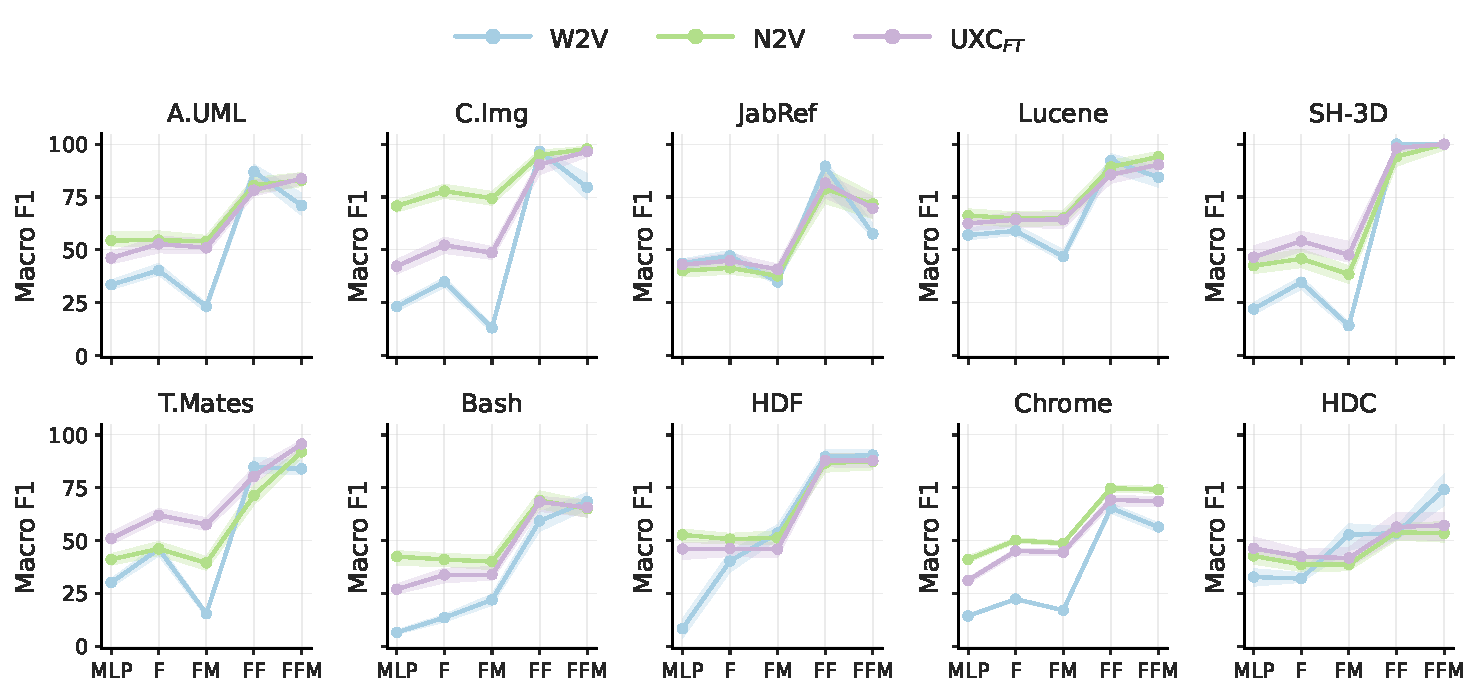
\includegraphics[width=0.93\textwidth]{Images/RQ2_lineplot_f1_macro.pdf}
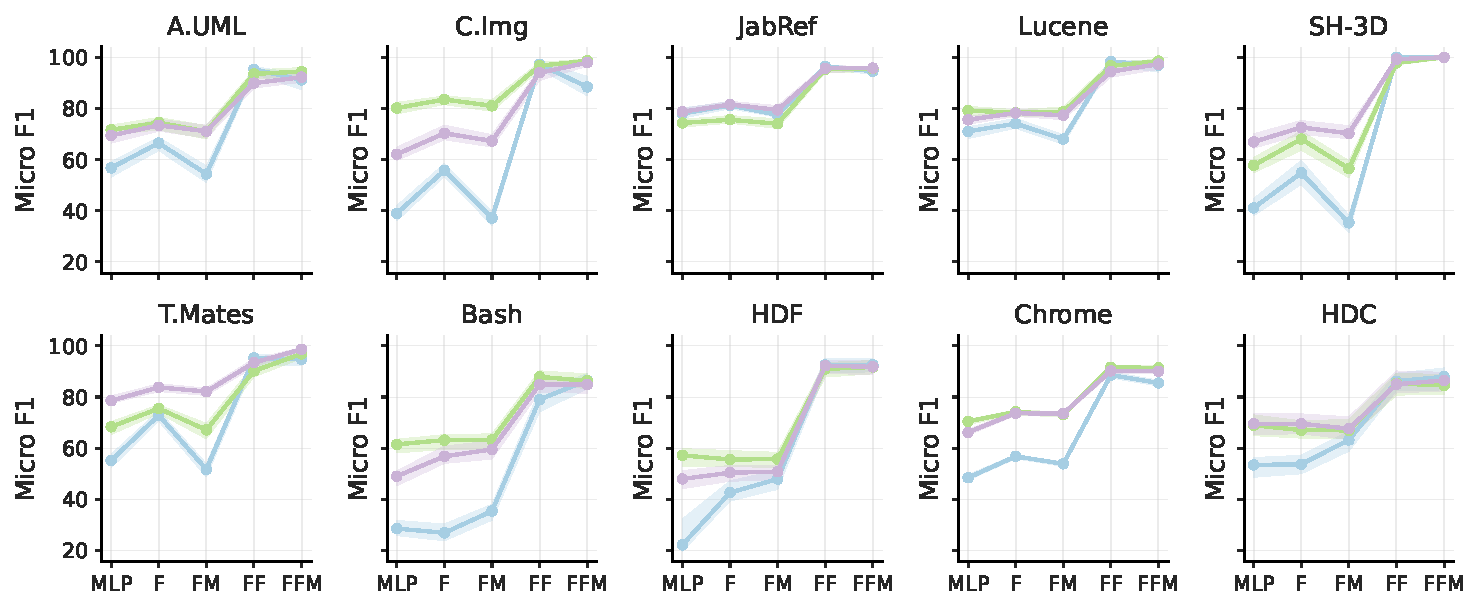
\includegraphics[width=0.93\textwidth]{Images/RQ2_lineplot_f1_micro.pdf}
\caption{Median macro-F1 (top) and micro-F1 (bottom) for each representation, per system, across the MLP and HGT with increasing graph structure (F, FF, FM, FFM). Shaded areas denote interquartile ranges across the 100 runs. \label{fig:rq2_lineplot}}
\end{figure*}
\begin{table*}[t]
\centering
\caption{Change in macro- and micro-F1 as graph structure is added, by representation. Each row compares the later configuration with the earlier one. Each cell gives the median difference across ten systems in F1 points, followed in parentheses by the number of systems with a positive difference and the numbers of significant positive and negative differences. Shading marks the median difference: blue for gains, purple for losses, and darker for larger changes.\label{tab:rq2_steps}}
\begin{adjustbox}{max width=\textwidth}
\setlength{\tabcolsep}{12pt}
\renewcommand{\arraystretch}{1.2}
\begin{tabular}{lrrrrrr}
\toprule
& \multicolumn{2}{c}{W2V} & \multicolumn{2}{c}{N2V} & \multicolumn{2}{c}{\ft{}} \\
\cmidrule(lr){2-3}\cmidrule(lr){4-5}\cmidrule(lr){6-7}
Step & Macro F1 & Micro F1 & Macro F1 & Micro F1 & Macro F1 & Micro F1 \\
\midrule
F $-$ MLP & \gc{45}+1.6 (6; 6/3) & \gc{45}+1.2 (6; 6/2) & \rc{45}$-$2.9 (1; 1/5) & \rc{70}$-$3.2 (2; 2/6) & \gc{45}+2.9 (8; 4/1) & \gc{25}+0.9 (7; 3/1) \\
FM $-$ F & \gc{45}+1.5 (6; 5/3) & \gc{45}+2.6 (7; 6/3) & \gc{25}+0.9 (6; 4/0) & \gc{45}+2.3 (7; 6/2) & \gc{45}+1.5 (7; 2/2) & \gc{45}+1.8 (8; 6/2) \\
FFM $-$ FF & \gc{100}+11.2 (10; 10/0) & \gc{70}+4.5 (10; 9/0) & \gc{70}+3.3 (8; 5/1) & \gc{45}+2.5 (8; 5/0) & \gc{70}+4.4 (8; 7/0) & \gc{45}+2.5 (10; 6/0) \\
FF $-$ F & \gc{100}+32.9 (10; 10/0) & \gc{100}+33.7 (10; 10/0) & \gc{100}+18.1 (10; 10/0) & \gc{100}+16.7 (10; 10/0) & \gc{100}+27.9 (10; 10/0) & \gc{100}+19.8 (10; 10/0) \\
FFM $-$ FM & \gc{100}+47.2 (10; 10/0) & \gc{100}+37.6 (10; 10/0) & \gc{100}+17.4 (10; 10/0) & \gc{100}+16.9 (10; 10/0) & \gc{100}+36.5 (10; 10/0) & \gc{100}+22.2 (10; 10/0) \\
\bottomrule
\end{tabular}
\end{adjustbox}
\end{table*}

% \begin{table*}[t]
% \centering
% \caption{Changes in Macro and F1 as graph structure is added, by representation. Rows compare the later configuration with the earlier one. $\Delta$ is the median difference across nine systems; $+$ve counts positive differences; $\uparrow/\downarrow$ gives the numbers of significant positive and negative differences, respectively (Wilcoxon signed-rank test, Holm-adjusted, $\alpha=0.05$). Shading marks $\Delta$: blue for gains, purple for losses, darker for larger changes.\label{tab:rq2_steps}}
% \begin{adjustbox}{max width=\textwidth}
% \large
% \begin{tabular}{lrrrrrrrrrrrrrrrrrrr}
% \toprule
% & \multicolumn{6}{c}{W2V} & \multicolumn{6}{c}{N2V} & \multicolumn{6}{c}{\ft{}} \\
% \cmidrule(lr){2-7}\cmidrule(lr){8-13}\cmidrule(lr){14-19}
% & \multicolumn{3}{c}{Macro F1} & \multicolumn{3}{c}{Micro F1}
% & \multicolumn{3}{c}{Macro F1} & \multicolumn{3}{c}{Micro F1}
% & \multicolumn{3}{c}{Macro F1} & \multicolumn{3}{c}{Micro F1} \\
% \cmidrule(lr){2-4}\cmidrule(lr){5-7}
% \cmidrule(lr){8-10}\cmidrule(lr){11-13}
% \cmidrule(lr){14-16}\cmidrule(lr){17-19}
% Step
% & $\Delta$ & $+$ve & $\uparrow/\downarrow$
% & $\Delta$ & $+$ve & $\uparrow/\downarrow$
% & $\Delta$ & $+$ve & $\uparrow/\downarrow$
% & $\Delta$ & $+$ve & $\uparrow/\downarrow$
% & $\Delta$ & $+$ve & $\uparrow/\downarrow$
% & $\Delta$ & $+$ve & $\uparrow/\downarrow$ \\
% \midrule
% F $-$ MLP
% & \gc{45}+1.8 & 6 & 6/2 & \gc{45}+1.5 & 6 & 6/3
% & \rc{45}$-$2.7 & 1 & 1/5 & \rc{45}$-$2.1 & 2 & 2/5
% & \gc{70}+3.7 & 7 & 6/1 & \gc{45}+1.2 & 7 & 7/1 \\
% FM $-$ F
% & \gc{25}+0.5 & 5 & 5/4 & \gc{45}+2.7 & 6 & 6/3
% & \gc{25}+0.1 & 5 & 3/1 & \gc{45}+1.5 & 6 & 6/3
% & \gc{45}+1.5 & 6 & 6/2 & \gc{45}+1.6 & 7 & 7/2 \\
% FFM $-$ FF
% & \gc{100}+10.1 & 9 & 9/0 & \gc{70}+4.0 & 9 & 9/0
% & \gc{45}+1.9 & 7 & 4/1 & \gc{45}+2.0 & 7 & 5/1
% & \gc{70}+3.6 & 7 & 7/0 & \gc{45}+2.4 & 9 & 9/0 \\
% FF $-$ F
% & \gc{100}+29.9 & 9 & 9/0 & \gc{100}+38.7 & 9 & 9/0
% & \gc{100}+19.0 & 9 & 9/0 & \gc{100}+16.4 & 9 & 9/0
% & \gc{100}+27.7 & 9 & 9/0 & \gc{100}+20.6 & 9 & 9/0 \\
% FFM $-$ FM
% & \gc{100}+45.5 & 9 & 9/0 & \gc{100}+38.8 & 9 & 9/0
% & \gc{100}+18.5 & 9 & 9/0 & \gc{100}+18.7 & 9 & 9/0
% & \gc{100}+35.9 & 9 & 9/0 & \gc{100}+20.8 & 9 & 9/0 \\
% \bottomrule
% \end{tabular}
% \end{adjustbox}
% \end{table*}

%_______________

\parg{File-level HGT versus the MLP.} Moving from the MLP to file-level HGT improves Word2Vec and \ft{} more than Node2Vec. For Word2Vec and \ft{}, F improves the median macro-F1 by 7.5 and 6.7 points and the median micro-F1 by 9.0 and 4.6 points, with positive differences on nine systems for each representation and metric. Word2Vec has no significant loss, and \ft{} has one, on HDC macro-F1. For Node2Vec, the medians change by 0.8 and 2.2 points, with positive differences on six and seven systems. Significant losses occur on Lucene and HDC for both metrics and on HDF for macro-F1, but significant gains still outnumber them (five to three on macro-F1, seven to two on micro-F1).

\parg{Member-level context.} Adding member nodes to F lowers the median macro-F1 by 12.2 points for Word2Vec and by 1.2 points for both Node2Vec and \ft{}, and the median micro-F1 by 4.9, 1.3, and 1.8 points. The decline is largest for Word2Vec, where all ten differences have large effects. Significant losses outnumber significant gains for all three representations: on macro-F1, seven systems decline significantly for Word2Vec, five for Node2Vec, and six for \ft{}, against significant gains on three, none, and one. Adding member nodes also changes how features enter the model, depending on the representation (Section~\ref{sec:node_features}); with \ft{}, for example, member vectors come from an encoder fine-tuned on file-level text only. These results therefore describe the evaluated member configuration and not member information in general.

\parg{Folder-level context.}
Adding folder nodes produces the largest and most consistent changes. FF improves over F, and FFM improves over FM, on both metrics for every system and representation. All 120 system--representation--metric comparisons are significant with a large effect. Across the three representations, the median macro-F1 gains range from 25.6 to 44.4 points for FF $-$ F and from 28.9 to 43.0 points for FFM $-$ FM. The corresponding micro-F1 gains range from 16.5 to 32.1 points and from 20.6 to 39.9 points. Each comparison improves in at least 96 of the 100 paired runs.
 
Within the folder-containing configurations, the effect of adding member nodes depends on the representation. FFM improves macro-F1 over FF on six systems each for Node2Vec and \ft{}, with median gains of 1.6 and 1.3 points, but on only three systems for Word2Vec, with a median loss of 4.4 points. For micro-F1, it improves seven, seven, and three systems for Node2Vec, \ft{}, and Word2Vec, with median changes of $+0.8$, $+1.1$, and $-1.0$ points. Significant macro-F1 losses occur on five systems for Word2Vec and on JabRef, Bash, and Chrome for both Node2Vec and \ft{}. For micro-F1, Node2Vec loses significantly only on Bash, and \ft{} on no system.


\parg{Folder nodes and the directory baseline.\label{sec:directory_errors}}
The large gains from adding folder nodes show that directory organization is informative for the evaluated mappings. To examine whether these gains also help files misclassified by directory information alone, we compare FM and FFM with \ft{} features against the directory hierarchy baseline of Section~\ref{sec:dir_predictor}.  FM and FFM differ only in the inclusion of folder nodes, allowing us to compare their performance with and without folder information. Table~\ref{tab:dir_baseline} gives the accuracy of the baseline, FM, and FFM per system, and the accuracy of FM and FFM on the files the baseline gets wrong.

\begin{table}[!htb]
\centering
\small
\caption{Accuracy (\%) of the directory baseline (Dir.) and of HGT with \ft{} features on FM and FFM, median over 100 runs. $n$ is the median number of test files misclassified by the baseline per split; the FM and FFM columns under it report median accuracy on those files over splits with at least one baseline error. Dashes (--) indicate omitted values for systems with no baseline errors in most or all splits. Purity is the share of all files that belong to the majority module of their directory.\label{tab:dir_baseline}}
\begin{adjustbox}{max width=\linewidth}
\begin{tabular}{lrrrrrrr}
\toprule
& \multicolumn{3}{c}{Accuracy} & \multicolumn{3}{c}{Files the baseline gets wrong} & \\
\cmidrule(lr){2-4}\cmidrule(lr){5-7}
System & Dir. & FM & FFM & $n$ & FM & FFM & Purity \\
\midrule
A.UML   & 98.5  & 71.0 & 92.2  & 11   & 9.1  & 21.7 & 100.0 \\
C.Img   & 100.0 & 67.3 & 97.9  & 0    & --   & --   & 100.0 \\
JabRef  & 97.2  & 79.4 & 95.8  & 27   & 45.3 & 26.3 & 99.1  \\
Lucene  & 91.5  & 77.4 & 97.3  & 85.5 & 52.9 & 86.9 & 100.0 \\
SH-3D   & 100.0 & 70.3 & 100.0 & 0    & --   & --   & 100.0 \\
T.Mates & 100.0 & 82.1 & 98.6  & 0    & --   & --   & 100.0 \\
Bash    & 91.8  & 59.5 & 84.8  & 21   & 24.6 & 26.1 & 91.8  \\
HDF     & 93.4  & 50.8 & 91.8  & 8    & 27.3 & 50.0 & 100.0 \\
Chrome  & 96.8  & 73.5 & 90.0  & 574  & 19.8 & 20.0 & 99.9  \\
HDC     & 89.1  & 67.6 & 86.5  & 19   & 20.0 & 12.5 & 96.1  \\
\bottomrule
\end{tabular}
\end{adjustbox}
\end{table}
The baseline reaches 89 to 100\% accuracy on every system. Without folder nodes, FM is 14 to 43 points below it. With folder nodes, FFM is within 3 points of the baseline on six systems and within 7 points on A.UML, Bash, and Chrome; it exceeds the baseline only on Lucene. Adding folder nodes therefore brings FFM close to the accuracy of the directory hierarchy baseline on most systems.

Directory membership closely matches module membership: on eight systems, 99 to 100\% of files belong to the majority module of their directory, and only Bash (91.8\%) and HDC (96.1\%) have lower purity. Files that depart from the majority module of their directory are therefore rare on most systems, which limits what the analysis can show about them.

On the files the baseline gets wrong, FFM gets most of them wrong on A.UML, JabRef, Bash, Chrome, and HDC, about 50\% on HDF, and most of them right only on Lucene. Compared with FM, FFM is more accurate on these files on A.UML, HDF, and Lucene, similar on Bash and Chrome, and less accurate on JabRef and HDC. JabRef shows why a higher overall accuracy is not sufficient: FFM improves over FM overall (79.4\% to 95.8\%), but its accuracy on these files falls (45.3\% to 26.3\%). This analysis does not isolate files whose module differs from the majority module of their directory, so it does not show how well FFM handles such exceptions.

\begin{GrayBox}{Answer to RQ2.}
The effect on mapping performance depends on what is added and on the representation. Moving from the MLP to file-level HGT improves Word2Vec and \ft{} more than Node2Vec. Member nodes give no consistent gain and often lower performance, most strongly for Word2Vec. Folder nodes provide the largest gains, improving performance on all ten systems for all three representations with significant large effects. However, the directory hierarchy alone achieves accuracy similar to FFM on most systems. On the files misclassified by that baseline, FFM is mostly incorrect on most systems, and on some it is less accurate than FM. Strong folder-based scores therefore do not establish reliable performance on directory-baseline errors or on files whose directory location is insufficient or misleading.
\end{GrayBox}
% ========================================
% ----------------- RQ3 ------------------
% ========================================
\subsection{Comparing Predictors and Dependency Direction (RQ3)\label{sec:rq3}}

RQ2 shows that the effect of graph context depends on the representation, configuration, and system. However, its comparison of the MLP with file-level HGT changes both the predictor and the availability of dependency messages. RQ3 therefore compares each predictor with dependency neighbors disabled and enabled, using HGT, GAT, and a neighbor MLP (\mlp{}). It also compares directed and undirected aggregation to examine whether the benefit depends on how dependency neighbors are aggregated. We evaluate all three predictors with all four input representations.

Differences are paired changes in F1 points, enabled minus disabled; positive values favor neighbor information. For direction, differences are undirected minus directed; positive values favor undirected neighbors. We report the median paired difference over the 100 splits. With neighbors disabled, the neighbor MLP reduces to the MLP of RQ1, and GAT and HGT receive no dependency messages.

\parg{How does the benefit of dependency neighbors vary across predictors and representations?} Table~\ref{tab:rq3_reps} shows the change in F1 when neighbor information is enabled, for each predictor and input representation. With undirected neighbors, the median change is positive in every cell on both metrics. GAT and the \mlp{} improve on at least eight systems in every cell and are never significantly lower, whereas HGT gains least with every representation and is significantly lower on a few systems with Node2Vec and Word2Vec. With directed neighbors, the median macro-F1 is lower with Node2Vec for all three predictors, by 0.6 to 2.8 points, and significant losses occur on up to six systems. For GAT and the \mlp{}, the gain from undirected neighbors is smallest with Node2Vec and largest with \zs{}.

This comparison differs from RQ2, where file-level message passing (F) is compared with the MLP, which changes the predictor together with the available structure. Here the predictor is fixed, and dependency neighbors are enabled and disabled, so a gain of F over the MLP does not imply that HGT benefits from dependency neighbors. With Node2Vec, for example, F raises the median macro-F1 over the MLP, whereas HGT with directed neighbors is lower than HGT without neighbors.

\begin{table*}[t]
\centering
\caption{Changes in F1 from enabling neighbor information (D$-$off, UD$-$off) and switching from directed to undirected aggregation (UD$-$D), by model and input representation. Each cell reports the median across ten systems of the per-system median paired change over runs, in F1 points. Parentheses follow the format (systems with a positive median change; significant gains/significant losses). D: directed (source-to-target); UD: undirected; off: neighbor information disabled. Blue shading indicates gains and purple indicates losses, with darker shades indicating larger magnitudes.\label{tab:rq3_reps}}

\begin{adjustbox}{max width=\textwidth}
\renewcommand{\arraystretch}{1.1}
\normalsize
\begin{tabular}{llrrrrrrrr}
\toprule
& & \multicolumn{2}{c}{N2V} & \multicolumn{2}{c}{W2V} & \multicolumn{2}{c}{\zs{}} & \multicolumn{2}{c}{\ft{}} \\
\cmidrule(lr){3-4}\cmidrule(lr){5-6}\cmidrule(lr){7-8}\cmidrule(lr){9-10}
Model & Contrast & Macro F1 & Micro F1 & Macro F1 & Micro F1 & Macro F1 & Micro F1 & Macro F1 & Micro F1 \\
\midrule
\multirow{3}{*}{HGT} & D$-$off & \rc{25}$-$0.6 (4; 4/6) & \gc{45}+1.6 (6; 6/4) & \gc{25}+0.2 (5; 4/5) & \gc{45}+1.8 (7; 7/3) & \gc{45}+1.6 (9; 7/0) & \gc{45}+2.7 (10; 10/0) & \gc{25}+0.7 (7; 6/3) & \gc{45}+1.8 (8; 8/0) \\
 & UD$-$off & \gc{25}+0.5 (8; 5/2) & \gc{25}+0.8 (9; 8/0) & \gc{45}+2.9 (7; 7/3) & \gc{70}+4.5 (8; 8/2) & \gc{45}+1.8 (10; 10/0) & \gc{45}+2.5 (10; 10/0) & \gc{25}+0.9 (10; 8/0) & \gc{45}+1.6 (10; 10/0) \\
 & UD$-$D & \gc{25}+0.3 (6; 5/4) & \gc{25}+0.1 (5; 3/4) & \gc{25}+0.7 (7; 4/3) & \gc{45}+1.5 (6; 5/4) & \rc{25}0.0 (5; 4/3) & \gc{25}+0.1 (5; 5/4) & \gc{25}+0.6 (6; 5/3) & \gc{25}+0.2 (5; 4/4) \\
\addlinespace[3pt]

\multirow{3}{*}{GAT} & D$-$off & \rc{45}$-$2.8 (4; 3/6) & \rc{25}$-$0.8 (3; 2/5) & \gc{45}+1.5 (8; 6/2) & \gc{45}+2.4 (7; 7/1) & \gc{70}+3.8 (10; 9/0) & \gc{100}+6.2 (10; 10/0) & \gc{25}+0.7 (6; 4/2) & \gc{45}+2.2 (8; 7/1) \\
 & UD$-$off & \gc{45}+1.4 (9; 8/0) & \gc{45}+1.4 (10; 10/0) & \gc{70}+5.6 (8; 7/0) & \gc{100}+6.7 (8; 8/0) & \gc{100}+8.2 (10; 10/0) & \gc{100}+9.5 (10; 10/0) & \gc{70}+3.8 (10; 8/0) & \gc{70}+4.1 (10; 10/0) \\
 & UD$-$D & \gc{70}+3.8 (7; 6/2) & \gc{45}+2.2 (8; 8/1) & \gc{45}+1.9 (7; 5/3) & \gc{45}+1.6 (7; 5/3) & \gc{70}+3.3 (6; 6/4) & \gc{45}+2.2 (6; 6/2) & \gc{45}+3.0 (6; 6/4) & \gc{45}+1.3 (7; 6/1) \\
\addlinespace[3pt]

\multirow{3}{*}{\mlp{}} & D$-$off & \rc{25}$-$0.6 (4; 4/5) & \gc{25}+0.8 (6; 5/4) & \gc{70}+3.4 (9; 9/1) & \gc{45}+2.7 (9; 8/1) & \gc{70}+4.8 (8; 7/1) & \gc{70}+5.1 (9; 9/0) & \gc{45}+2.8 (7; 6/2) & \gc{45}+2.9 (7; 7/2) \\
 & UD$-$off & \gc{45}+1.2 (10; 8/0) & \gc{45}+1.2 (9; 8/0) & \gc{70}+5.1 (10; 10/0) & \gc{70}+4.9 (10; 10/0) & \gc{100}+7.7 (10; 10/0) & \gc{100}+7.3 (10; 10/0) & \gc{70}+5.8 (10; 10/0) & \gc{70}+4.6 (10; 10/0) \\
 & UD$-$D & \gc{45}+1.6 (6; 6/4) & \gc{25}+0.4 (6; 5/3) & \gc{45}+1.3 (6; 6/3) & \gc{45}+1.9 (6; 6/2) & \gc{70}+3.5 (6; 6/4) & \gc{45}+2.5 (6; 6/4) & \gc{70}+3.1 (6; 6/3) & \gc{45}+1.3 (7; 7/3) \\
\bottomrule
\end{tabular}
\end{adjustbox}
\end{table*}



 % \begin{table*}[thb]
% \centering
% \caption{Change in macro- and micro-F1 when neighbor information is switched on, by input vector. $\Delta$ is the median difference across nine systems; $+$ve counts positive differences; $\uparrow/\downarrow$ gives the numbers of significant positive and negative differences, respectively (Wilcoxon signed-rank test, Holm-adjusted, $\alpha=0.05$). Shading marks $\Delta$: blue for gains, purple for losses, darker for larger changes.\label{tab:rq3_reps}}
% \begin{adjustbox}{max width=\textwidth}
% \large
% \begin{tabular}{llrrrrrrrrrrrrrrrrrrrrrrrr}
% \toprule
% & & \multicolumn{6}{c}{N2V} & \multicolumn{6}{c}{W2V} & \multicolumn{6}{c}{\zs{}} & \multicolumn{6}{c}{\ft{}} \\
% \cmidrule(lr){3-8}\cmidrule(lr){9-14}\cmidrule(lr){15-20}\cmidrule(lr){21-26}
% & & \multicolumn{3}{c}{Macro F1} & \multicolumn{3}{c}{Micro F1}
% & \multicolumn{3}{c}{Macro F1} & \multicolumn{3}{c}{Micro F1}
% & \multicolumn{3}{c}{Macro F1} & \multicolumn{3}{c}{Micro F1}
% & \multicolumn{3}{c}{Macro F1} & \multicolumn{3}{c}{Micro F1} \\
% \cmidrule(lr){3-5}\cmidrule(lr){6-8}
% \cmidrule(lr){9-11}\cmidrule(lr){12-14}
% \cmidrule(lr){15-17}\cmidrule(lr){18-20}
% \cmidrule(lr){21-23}\cmidrule(lr){24-26}
% Model & Sch.
% & $\Delta$ & $+$ve & $\uparrow/\downarrow$
% & $\Delta$ & $+$ve & $\uparrow/\downarrow$
% & $\Delta$ & $+$ve & $\uparrow/\downarrow$
% & $\Delta$ & $+$ve & $\uparrow/\downarrow$
% & $\Delta$ & $+$ve & $\uparrow/\downarrow$
% & $\Delta$ & $+$ve & $\uparrow/\downarrow$
% & $\Delta$ & $+$ve & $\uparrow/\downarrow$
% & $\Delta$ & $+$ve & $\uparrow/\downarrow$ \\
% \midrule

% HGT & sup. & \rc{70}$-$4.6 & 1 & 0/5 & \rc{45}$-$2.0 & 2 & 2/4 & \rc{70}$-$3.9 & 2 & 2/7 & \rc{45}$-$1.0 & 2 & 2/5 & \rc{45}$-$1.2 & 4 & 1/2 & \rc{25}$-$0.2 & 4 & 2/1 & \rc{70}$-$3.9 & 4 & 0/3 & \rc{45}$-$1.7 & 3 & 1/3 \\
%  & self. & \rc{70}$-$4.8 & 0 & 0/5 & \rc{45}$-$2.4 & 3 & 1/4 & \rc{70}$-$3.6 & 2 & 2/7 & \rc{45}$-$2.0 & 3 & 2/5 & \rc{45}$-$1.3 & 2 & 0/0 & \gc{25}+0.2 & 5 & 1/1 & \rc{45}$-$2.2 & 2 & 0/3 & \rc{45}$-$1.2 & 3 & 1/2 \\
% \addlinespace[3pt]
% \multirow{2}{*}{\shortstack[l]{HGT\\-UT}} & sup. & \gc{25}+0.6 & 5 & 2/1 & \gc{25}+0.9 & 7 & 2/0 & \gc{45}+2.6 & 6 & 4/1 & \gc{70}+4.0 & 7 & 7/1 & \gc{45}+1.6 & 9 & 8/0 & \gc{70}+3.1 & 9 & 9/0 & \gc{25}+0.9 & 9 & 2/0 & \gc{45}+1.4 & 9 & 6/0 \\
%  & self. & \gc{25}+0.4 & 6 & 0/1 & \gc{45}+1.2 & 8 & 3/0 & \gc{45}+1.7 & 6 & 2/0 & \gc{70}+3.9 & 7 & 7/0 & \gc{45}+2.1 & 8 & 6/0 & \gc{70}+3.1 & 9 & 8/0 & \gc{45}+1.8 & 9 & 2/0 & \gc{45}+2.0 & 9 & 5/0 \\
% \addlinespace[3pt]
% GAT & sup. & \gc{45}+1.1 & 8 & 3/0 & \gc{45}+1.6 & 9 & 9/0 & \gc{70}+5.7 & 8 & 3/0 & \gc{100}+6.4 & 9 & 6/0 & \gc{100}+7.7 & 9 & 7/0 & \gc{100}+10.5 & 9 & 9/0 & \gc{70}+4.2 & 7 & 4/0 & \gc{70}+4.4 & 9 & 7/0 \\
%  & self. & \gc{70}+3.2 & 9 & 3/0 & \gc{45}+2.9 & 8 & 7/0 & \gc{70}+3.7 & 7 & 3/0 & \gc{100}+6.9 & 7 & 6/0 & \gc{100}+8.0 & 8 & 8/0 & \gc{100}+8.9 & 9 & 9/0 & \gc{70}+4.2 & 8 & 4/0 & \gc{70}+4.2 & 8 & 4/0 \\
% \addlinespace[3pt]
% MLP & sup. & \gc{25}+0.7 & 8 & 4/0 & \gc{45}+1.4 & 8 & 5/0 & \gc{70}+4.4 & 8 & 6/0 & \gc{70}+4.4 & 8 & 5/0 & \gc{100}+6.9 & 9 & 8/0 & \gc{70}+5.2 & 9 & 9/0 & \gc{70}+4.0 & 8 & 4/0 & \gc{70}+4.5 & 9 & 5/0 \\
%  & self. & \gc{45}+2.6 & 8 & 5/0 & \gc{45}+2.8 & 8 & 6/0 & \gc{70}+3.6 & 9 & 6/0 & \gc{70}+4.6 & 9 & 5/0 & \gc{100}+6.8 & 8 & 6/0 & \gc{100}+6.9 & 9 & 9/0 & \gc{100}+6.3 & 9 & 5/0 & \gc{70}+4.6 & 9 & 8/0 \\
% \bottomrule
% \end{tabular}
% \end{adjustbox}
% \end{table*}


% % --- Table B
% \begin{table*}[thb]
% \centering
% \caption{Change in macro- and micro-F1 when neighbor information is switched on, by input vector. $\Delta$ is the median difference across nine systems; $+$ve counts positive differences; $\uparrow/\downarrow$ gives the numbers of significant positive and negative differences, respectively (Wilcoxon signed-rank test, Holm-adjusted, $\alpha=0.05$). Shading marks $\Delta$: blue for gains, purple for losses, darker for larger changes.\label{tab:rq3_reps}}
% \begin{adjustbox}{max width=\textwidth}
% \large
% \begin{tabular}{llrrrrrrrrrrrrrrrrrr}
% \toprule
% & & \multicolumn{6}{c}{N2V} & \multicolumn{6}{c}{W2V} & \multicolumn{6}{c}{\ft{}} \\
% \cmidrule(lr){3-8}\cmidrule(lr){9-14}\cmidrule(lr){15-20}
% & & \multicolumn{3}{c}{Macro F1} & \multicolumn{3}{c}{Micro F1}
% & \multicolumn{3}{c}{Macro F1} & \multicolumn{3}{c}{Micro F1}
% & \multicolumn{3}{c}{Macro F1} & \multicolumn{3}{c}{Micro F1} \\
% \cmidrule(lr){3-5}\cmidrule(lr){6-8}
% \cmidrule(lr){9-11}\cmidrule(lr){12-14}
% \cmidrule(lr){15-17}\cmidrule(lr){18-20}
% Model & Sch.
% & $\Delta$ & $+$ve & $\uparrow/\downarrow$
% & $\Delta$ & $+$ve & $\uparrow/\downarrow$
% & $\Delta$ & $+$ve & $\uparrow/\downarrow$
% & $\Delta$ & $+$ve & $\uparrow/\downarrow$
% & $\Delta$ & $+$ve & $\uparrow/\downarrow$
% & $\Delta$ & $+$ve & $\uparrow/\downarrow$ \\
% \midrule

% HGT & sup. & \rc{70}$-$4.6 & 1 & 0/5 & \rc{45}$-$2.0 & 2 & 2/4 & \rc{70}$-$3.9 & 2 & 2/7 & \rc{45}$-$1.0 & 2 & 2/5 & \rc{70}$-$3.9 & 4 & 0/3 & \rc{45}$-$1.7 & 3 & 1/3 \\
%  & self. & \rc{70}$-$4.8 & 0 & 0/5 & \rc{45}$-$2.4 & 3 & 1/4 & \rc{70}$-$3.6 & 2 & 2/7 & \rc{45}$-$2.0 & 3 & 2/5 & \rc{45}$-$2.2 & 2 & 0/3 & \rc{45}$-$1.2 & 3 & 1/2 \\
% \addlinespace[3pt]
% \uhgt{} & sup. & \gc{25}+0.6 & 5 & 2/1 & \gc{25}+0.9 & 7 & 2/0 & \gc{45}+2.6 & 6 & 4/1 & \gc{70}+4.0 & 7 & 7/1 & \gc{25}+0.9 & 9 & 2/0 & \gc{45}+1.4 & 9 & 6/0 \\
%  & self. & \gc{25}+0.4 & 6 & 0/1 & \gc{45}+1.2 & 8 & 3/0 & \gc{45}+1.7 & 6 & 2/0 & \gc{70}+3.9 & 7 & 7/0 & \gc{45}+1.8 & 9 & 2/0 & \gc{45}+2.0 & 9 & 5/0 \\
% \addlinespace[3pt]
% GAT & sup. & \gc{45}+1.1 & 8 & 3/0 & \gc{45}+1.6 & 9 & 9/0 & \gc{70}+5.7 & 8 & 3/0 & \gc{100}+6.4 & 9 & 6/0 & \gc{70}+4.2 & 7 & 4/0 & \gc{70}+4.4 & 9 & 7/0 \\
%  & self. & \gc{70}+3.2 & 9 & 3/0 & \gc{45}+2.9 & 8 & 7/0 & \gc{70}+3.7 & 7 & 3/0 & \gc{100}+6.9 & 7 & 6/0 & \gc{70}+4.2 & 8 & 4/0 & \gc{70}+4.2 & 8 & 4/0 \\
% \addlinespace[3pt]
% MLP & sup. & \gc{25}+0.7 & 8 & 4/0 & \gc{45}+1.4 & 8 & 5/0 & \gc{70}+4.4 & 8 & 6/0 & \gc{70}+4.4 & 8 & 5/0 & \gc{70}+4.0 & 8 & 4/0 & \gc{70}+4.5 & 9 & 5/0 \\
%  & self. & \gc{45}+2.6 & 8 & 5/0 & \gc{45}+2.8 & 8 & 6/0 & \gc{70}+3.6 & 9 & 6/0 & \gc{70}+4.6 & 9 & 5/0 & \gc{100}+6.3 & 9 & 5/0 & \gc{70}+4.6 & 9 & 8/0 \\
% \bottomrule
% \end{tabular}
% \end{adjustbox}
% \end{table*}


\parg{Does the direction of neighbor aggregation matter?} Undirected aggregation gives the higher median in almost every cell of Table~\ref{tab:rq3_reps}, which raises the question of whether it is better on every system. Figure~\ref{fig:rq3_direction} compares the two directions per system. It is not: the change from directed to undirected aggregation is positive on only five to eight systems per cell, and significant changes occur in both directions. On macro-F1, SH-3D, T.Mates, and JabRef score higher with directed aggregation in all 12 cells, and C.Img in eight. Lucene, Bash, Chrome, and HDC score higher with undirected aggregation in all 12 cells, and A.UML and HDF in 11. The differences reach 14.6 points for undirected aggregation (Bash, Word2Vec, \mlp{}) and 8.7 points for directed aggregation (T.Mates, Word2Vec, \mlp{}). Micro-F1 gives the same pattern for seven systems, whereas JabRef, C.Img, and A.UML are mixed. Undirected neighbors also add the reverse edges, so these results do not separate the direction of propagation from the larger neighborhood.

\begin{figure}[t]
\centering
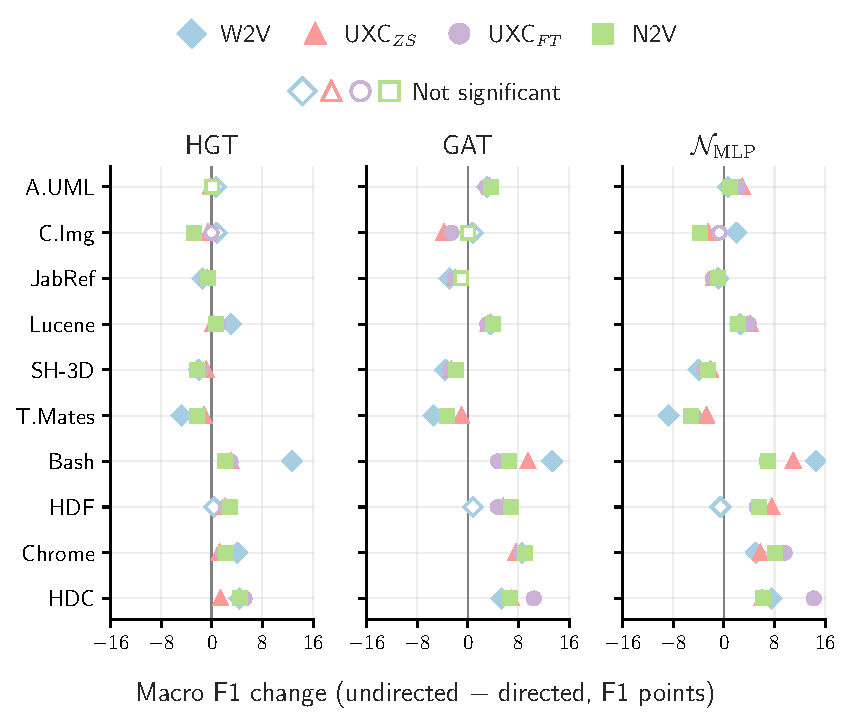
\includegraphics[width=1\columnwidth]{Images/rq3_direction_f1_macro.pdf}
\caption{Change in macro-F1, in F1 points, from directed to undirected aggregation (undirected $-$ directed) for each predictor and input representation; negative values mean directed aggregation scored higher. Each point is the median over 100 paired splits; hollow markers are not significant.\label{fig:rq3_direction}}
\end{figure}

\parg{Which predictor scores highest?} Figure~\ref{fig:rq3_agg} pools the ten systems with undirected neighbors: each point is the median of one system and the boxes show the spread across systems. GAT has the highest median macro-F1 with every representation and the highest median micro-F1 with every representation except Node2Vec, where HGT is marginally higher. GAT also scores highest most often: in each split we count which of the four predictors scores highest, and GAT has the largest share of wins, averaged over systems, with every representation and on both metrics. All three predictors with neighborhood aggregation exceed the MLP without neighbors in every median comparison. As without neighbors, \ft{} has the highest median macro-F1 across systems for every predictor, with GAT and \ft{} giving the highest scores overall.

Most of the variation in F1 lies between systems and not between runs of one system. The choice of predictor matters most for Word2Vec and \zs{}, the two representations without dependency information, and less for Node2Vec and \ft{}.

\begin{figure*}[h]
\centering
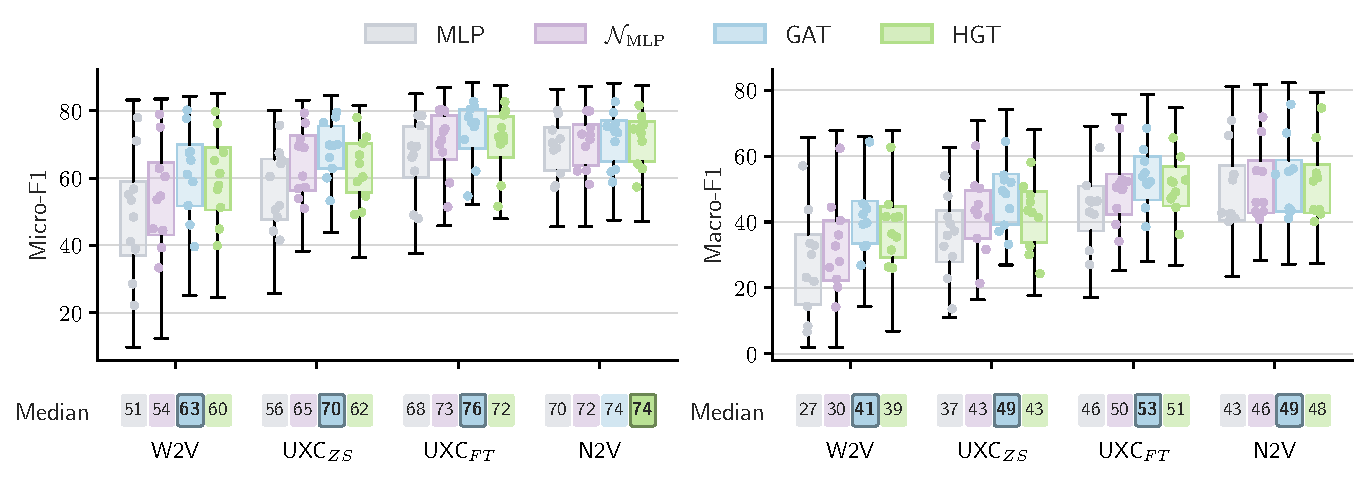
\includegraphics[width=0.98\textwidth]{Images/rq3_fig_compare_undirected.pdf}
\caption{Micro-F1 (left) and macro-F1 (right) of the MLP, \mlp{}, GAT, and HGT with undirected neighbors, by input representation. Each point is the median of one system over 100 runs; boxes show the spread across systems, and the values below are the median of medians across systems, with the highest in each group in bold.\label{fig:rq3_agg}}
\end{figure*}

\begin{GrayBox}{Answer to RQ3.}
Dependency neighbors do not benefit all predictors equally. With undirected aggregation, median changes are positive for every predictor and representation, but GAT and the \mlp{} improve more consistently across systems than HGT, which shows significant losses in some cases. Directed aggregation is less reliable, particularly with Node2Vec, where median macro-F1 decreases for all three predictors. Although undirected aggregation generally gives larger gains, it is not preferable on every system: several systems consistently favor directed aggregation across predictors and representations. These comparisons also change neighborhood size, so they do not isolate direction alone. With undirected neighbors, GAT has the highest median macro-F1 across systems for every representation, and \ft{} remains the strongest representation by this measure for every predictor.
\end{GrayBox}
% ================
% 3b_discussion
% ================
\section{Discussion\label{sec:discussion}}

The research questions examine where architectural signal resides and how a mapping model can use it. RQ1 compares what file representations encode before message passing, RQ2 adds file, member, and folder context and compares the folder gains with a directory-based rule, and RQ3 examines how the predictor and the direction in which it aggregates dependency neighbors change what they contribute. This section considers the three together and states the conditions under which they hold.

\parg{Dependency information in file representations.}
RQ1~\ref{sec:rq1} compares file representations before the predictor exchanges information between linked files, so the results reflect the architectural information encoded in each representation. Node2Vec, which is learned from the dependency graph alone, without labels, has the highest median micro-F1 and macro-F1 on six of the ten systems. Fine-tuned UniXcoder significantly improves over its zero-shot counterpart on micro-F1 on all ten systems and on macro-F1 on nine. Since the zero-shot encoder receives no dependency signal, this shows that fine-tuning on dependency-derived pairs adds information beyond that of pretrained code representations alone. Dependency information can therefore provide useful architectural signal before a predictor combines information across dependency links, either by encoding graph position directly in Node2Vec or by adapting a contextual code representation through dependency-guided fine-tuning.

The usefulness of this signal varies with the relation between dependency structure and the reference architecture. Node2Vec's micro-F1 is lower on the three least homophilic systems, SH-3D, HDF, and T.Mates (Table~\ref{tab:datasets}), with a median of $58$ compared with $72$ on the remaining seven. When dependencies frequently cross module boundaries, random walks may place files from different modules in similar structural neighborhoods, limiting the module-discriminating information available to Node2Vec. Homophily is computed from the reference mapping and is therefore unavailable before a mapping exists; it is used here to interpret the observed pattern, not to select a representation in practice.

Fine-tuned UniXcoder shows a different pattern on the low-homophily systems. Its median micro-F1 is $67$ on SH-3D, HDF, and T.Mates, compared with $69.5$ on the remaining seven. It exceeds Node2Vec by $9$ and $10$ micro-F1 points on SH-3D and T.Mates, which combine low homophily with the highest average degrees, $\langle k \rangle$ of $23.43$ and $22.90$. In these systems, dependency neighborhoods may span several modules, while the code content represented by UniXcoder can provide complementary evidence within such mixed neighborhoods. HDF is the exception: Node2Vec remains ahead of \ft{} ($57$ versus $48$ micro-F1), although every representation performs comparatively poorly on this system.

The two representations without dependency information, Word2Vec and zero-shot UniXcoder, show no consistent ordering. Their weaker overall results reinforce that the advantage of Node2Vec and \ft{} is associated with dependency information rather than with the use of a graph embedding or a code encoder alone.

The RQ2 and RQ3 comparison concerns a different use of dependencies. While Node2Vec learns file vectors from unlabeled random walks, the neighbor-based predictors use dependency links while learning the mapping from the available labels. The results show that useful dependency information in an input representation does not by itself determine whether this additional neighbor use helps: with N2V, directed aggregation lowers the median macro-F1 for all three predictors, whereas undirected aggregation raises it, and HGT gains least from neighbors with every representation. The effect therefore depends on how the predictor aggregates the neighborhood and in which direction.

\parg{Folder organization and architectural exceptions.}
The gains from adding folder nodes in RQ2 show that directory organization helps reproduce the reference mapping. However, extending a directory assignment is different from identifying files that depart from it. The directory analysis separates these cases by checking, on the files that a directory-based baseline gets wrong, which incorrect predictions of FM the folder nodes correct and which correct predictions they lose (Section~\ref{sec:directory_errors}).

Lucene and HDF mainly illustrate the first case. Their directories are pure under the reference mapping, and directory-baseline errors occur where the immediate directory has no labeled examples. Correcting these errors shows that a model can recover an assignment when local supervision is missing. It gives little evidence about conflicts between directory structure and architecture. Bash has mixed directories and therefore presents a different problem. JabRef shows why the distinction matters: adding folder context improves overall accuracy while losing more correct predictions on directory-baseline errors than it gains.

A mapping tool intended to identify architectural exceptions should therefore be evaluated on files that depart from their directory assignment, alongside overall accuracy. A rule-based directory baseline using only the initial labels provides a useful reference, but the counts compare FM with FFM on the baseline's errors and do not show how each model compares with the baseline on those files. Recovering assignments in directories without initial labels is useful, but does not establish that a model can identify files whose module assignment conflicts with their directory.

\parg{Dependency neighborhood processing and aggregation direction.}
RQ3 distinguishes dependency information encoded in file representations from its additional use during prediction. With undirected aggregation, dependency neighbors raise the median score for GAT, HGT, and the neighbor \mlp{} with every representation, including N2V and \ft{}, so dependency-informed initialization does not make neighbor access redundant. The gains are larger for W2V and \zs{}, which do not encode dependencies, than for N2V and \ft{}, which reinforces the RQ1 finding that dependencies provide signal beyond file content. HGT gains least with every representation and GAT scores highest in most comparisons, although the differences between predictors are small relative to the variation across systems. GAT and HGT differ in their attention formulation and parameterization, so the comparison does not isolate why GAT performs better. These findings concern the evaluated file-level predictors, not the usefulness of dependency types in general or the folder- and member-aware configurations.

The preferred direction of aggregation follows the system and not the predictor or the representation. SH-3D and T.Mates favor directed aggregation, and Lucene, Bash, Chrome, HDC, and HDF favor undirected aggregation, on both metrics. Undirected aggregation also adds the reverse edges, so the comparison does not isolate the direction of propagation from the larger neighborhood. With N2V, directed aggregation lowers the median macro-F1 for all three predictors. The N2V vectors were learned on the undirected dependency graph, which may make directed aggregation less consistent with the neighborhood that each vector encodes, but we did not test this.

\parg{Connectivity and neighbor information.}
Connectivity describes how much neighboring context is available, measured here by the average node degree, while homophily describes whether linked files share a module. Shallow message passing reaches only as far as its number of layers, so files with few neighbors provide little to aggregate, whereas Node2Vec can encode more distant context through random walks. Connectivity can therefore constrain additional message passing even when the initial structural representation remains useful.

Several results are consistent with this. With N2V and undirected aggregation, no predictor changes significantly on Bash and HDC, the two systems with the lowest average degree. T.Mates and SH-3D combine low homophily with among the highest average degrees, gain most from file-level message passing with N2V in RQ2, and favor directed aggregation in RQ3. Across systems, the advantage of undirected over directed aggregation decreases with the expected number of cross-module neighbors per file, $\langle k\rangle(1-H)$, more clearly than with homophily alone, although HDF, which has low homophily but a much lower average degree, does not follow this pattern. One reading is that reverse edges supply missing context for files with few neighbors but add mostly cross-module neighbors where files already have many. With ten systems and correlated descriptors, we cannot separate connectivity from homophily, system size, or label scarcity, and we did not test this.

\parg{Implications for evaluating mapping models.}
Evaluation should establish what the input representation already provides, then isolate neighbor access within a fixed predictor. Comparing a graph model with a graph-free MLP changes both the predictor and its access to structure; switching neighbors on and off within the same predictor tests whether that access helps.

Macro and micro F1 scores should be read together, since correctly mapping more files does not necessarily improve performance across modules. The directory analysis adds a further requirement: aggregate scores should be accompanied by evidence about files that depart from directory-based assignments. Together, these comparisons distinguish the contributions of input features, neighbor processing, and neighbor direction, while exposing limitations hidden by aggregate scores. These points concern the ten systems and the compared configurations and do not rank the signals or the predictors in general.

% _____________ 5_threats ________________
\section{Discussion\label{sec:discussion}}

The research questions examine where architectural signal resides and how a mapping model can use it. RQ1 compares what file representations encode before message passing, RQ2 adds file, member, and folder context and compares the folder gains with a directory-based rule, and RQ3 examines how the predictor and the direction in which it aggregates dependency neighbors change what they contribute. This section considers the three together and states the conditions under which they hold.

\parg{Dependency information in file representations.}
RQ1~\ref{sec:rq1} compares file representations before the predictor exchanges information between linked files, so the results reflect the architectural information encoded in each representation. Node2Vec, which is learned from the dependency graph alone, without labels, has the highest median micro-F1 and macro-F1 on six of the ten systems. Fine-tuned UniXcoder significantly improves over its zero-shot counterpart on micro-F1 on all ten systems and on macro-F1 on nine. Since the zero-shot encoder receives no dependency signal, this shows that fine-tuning on dependency-derived pairs adds information beyond that of pretrained code representations alone. Dependency information can therefore provide useful architectural signal before a predictor combines information across dependency links, either by encoding graph position directly in Node2Vec or by adapting a contextual code representation through dependency-guided fine-tuning.

The usefulness of this signal varies with the relation between dependency structure and the reference architecture. Node2Vec's micro-F1 is lower on the three least homophilic systems, SH-3D, HDF, and T.Mates (Table~\ref{tab:datasets}), with a median of $58$ compared with $72$ on the remaining seven. When dependencies frequently cross module boundaries, random walks may place files from different modules in similar structural neighborhoods, limiting the module-discriminating information available to Node2Vec. Homophily is computed from the reference mapping and is therefore unavailable before a mapping exists; it is used here to interpret the observed pattern, not to select a representation in practice.

Fine-tuned UniXcoder shows a different pattern on the low-homophily systems. Its median micro-F1 is $67$ on SH-3D, HDF, and T.Mates, compared with $69.5$ on the remaining seven. It exceeds Node2Vec by $9$ and $10$ micro-F1 points on SH-3D and T.Mates, which combine low homophily with the highest average degrees, $\langle k \rangle$ of $23.43$ and $22.90$. In these systems, dependency neighborhoods may span several modules, while the code content represented by UniXcoder can provide complementary evidence within such mixed neighborhoods. HDF is the exception: Node2Vec remains ahead of \ft{} ($57$ versus $48$ micro-F1), although every representation performs comparatively poorly on this system.

The two representations without dependency information, Word2Vec and zero-shot UniXcoder, show no consistent ordering. Their weaker overall results reinforce that the advantage of Node2Vec and \ft{} is associated with dependency information rather than with the use of a graph embedding or a code encoder alone.

The RQ2 and RQ3 comparison concerns a different use of dependencies. While Node2Vec learns file vectors from unlabeled random walks, the neighbor-based predictors use dependency links while learning the mapping from the available labels. The results show that useful dependency information in an input representation does not by itself determine whether this additional neighbor use helps: with N2V, directed aggregation lowers the median macro-F1 for all three predictors, whereas undirected aggregation raises it, and HGT gains least from neighbors with every representation. The effect therefore depends on how the predictor aggregates the neighborhood and in which direction.

\parg{Folder organization and architectural exceptions.}
The gains from adding folder nodes in RQ2 show that directory organization helps reproduce the reference mapping. However, extending a directory assignment is different from identifying files that depart from it. The directory analysis separates these cases by checking, on the files that a directory-based baseline gets wrong, which incorrect predictions of FM the folder nodes correct and which correct predictions they lose (Section~\ref{sec:directory_errors}).

Lucene and HDF mainly illustrate the first case. Their directories are pure under the reference mapping, and directory-baseline errors occur where the immediate directory has no labeled examples. Correcting these errors shows that a model can recover an assignment when local supervision is missing. It gives little evidence about conflicts between directory structure and architecture. Bash has mixed directories and therefore presents a different problem. JabRef shows why the distinction matters: adding folder context improves overall accuracy while losing more correct predictions on directory-baseline errors than it gains.

A mapping tool intended to identify architectural exceptions should therefore be evaluated on files that depart from their directory assignment, alongside overall accuracy. A rule-based directory baseline using only the initial labels provides a useful reference, but the counts compare FM with FFM on the baseline's errors and do not show how each model compares with the baseline on those files. Recovering assignments in directories without initial labels is useful, but does not establish that a model can identify files whose module assignment conflicts with their directory.

\parg{Dependency neighborhood processing and aggregation direction.}
RQ3 distinguishes dependency information encoded in file representations from its additional use during prediction. With undirected aggregation, dependency neighbors raise the median score for GAT, HGT, and the neighbor \mlp{} with every representation, including N2V and \ft{}, so dependency-informed initialization does not make neighbor access redundant. The gains are larger for W2V and \zs{}, which do not encode dependencies, than for N2V and \ft{}, which reinforces the RQ1 finding that dependencies provide signal beyond file content. HGT gains least with every representation and GAT scores highest in most comparisons, although the differences between predictors are small relative to the variation across systems. GAT and HGT differ in their attention formulation and parameterization, so the comparison does not isolate why GAT performs better. These findings concern the evaluated file-level predictors, not the usefulness of dependency types in general or the folder- and member-aware configurations.

The preferred direction of aggregation follows the system and not the predictor or the representation. SH-3D and T.Mates favor directed aggregation, and Lucene, Bash, Chrome, HDC, and HDF favor undirected aggregation, on both metrics. Undirected aggregation also adds the reverse edges, so the comparison does not isolate the direction of propagation from the larger neighborhood. With N2V, directed aggregation lowers the median macro-F1 for all three predictors. The N2V vectors were learned on the undirected dependency graph, which may make directed aggregation less consistent with the neighborhood that each vector encodes, but we did not test this.

\parg{Connectivity and neighbor information.}
Connectivity describes how much neighboring context is available, while homophily describes whether linked files share a module. Connectivity matters particularly for shallow message passing, whose reach is limited by the number of layers. Sparse neighborhoods restrict the features available for aggregation, whereas Node2Vec can encode more distant context through random walks. Connectivity can therefore constrain additional message passing even when the initial structural representation remains useful.

With N2V and undirected aggregation, no predictor changes significantly on Bash and HDC, the systems with the lowest average degree. This is consistent with limited local context reducing the benefit of neighbor aggregation, but does not establish connectivity as the cause. In contrast, T.Mates and SH-3D have low homophily but among the highest average degrees, and they are the systems with the largest N2V micro-F1 gains from file-level message passing in RQ2 ($+7.2$ and $+10.3$ points) and the systems that favor directed aggregation in RQ3. HDF has similarly low homophily but a much lower degree and no comparable gain. These observations suggest that connectivity is relevant to the context available for shallow message passing, but with ten systems and correlated descriptors we cannot separate connectivity from homophily, system size, or label scarcity, and we did not test this.

\parg{Implications for evaluating mapping models.}
Evaluation should establish what the input representation already provides, then isolate neighbor access within a fixed predictor. Comparing a graph model with a graph-free MLP changes both the predictor and its access to structure; switching neighbors on and off within the same predictor tests whether that access helps.

Macro and micro F1 scores should be read together, since correctly mapping more files does not necessarily improve performance across modules. The directory analysis adds a further requirement: aggregate scores should be accompanied by evidence about files that depart from directory-based assignments. Together, these comparisons distinguish the contributions of input features, neighbor processing, and neighbor direction, while exposing limitations hidden by aggregate scores. These points concern the ten systems and the compared configurations and do not rank the signals or the predictors in general.
% ___________ 6_conclusion ________________
\section{Conclusion\label{sec:conclusion}}
This study examines which implementation-level signals, including code text, static dependencies, folder organization, and member-level information, carry architectural information and how their representation and use affect code-to-architecture mapping on ten systems. We encode file information using lexical Word2Vec, structural Node2Vec, and contextual UniXcoder in zero-shot (\zs{}) and dependency-guided fine-tuned (\ft{}) variants, and evaluate these representations with MLP- and GNN-based predictors. Representations that encode dependencies, Node2Vec and \ft{}, outperform Word2Vec on most systems when evaluated with the MLP, whereas Word2Vec and \zs{}, which do not, differ from each other in both directions. Dependency-guided fine-tuning significantly improves mapping performance over \zs{} on at least nine of ten systems, although Node2Vec and \ft{} are each significantly stronger on different systems and no representation is best on every system. Folder nodes produce the largest and most consistent gains within HGT variants, but largely recover information already available to a directory rule using the initial labels and do not consistently improve the files on which that rule fails. Member nodes do not give consistent gains, and their effect cannot generally be separated from changes in feature construction and placement.

The controlled experiments distinguish dependency information encoded in file representations from its additional use during prediction by keeping the input representations fixed and switching dependency neighbors off, directed, or undirected for three predictors on all ten systems. With undirected aggregation, dependency neighbors raise the median score for GAT, HGT, and the neighbor \mlp{}, which concatenates own-file features with mean-neighbor features, across all four representations, with larger gains for Word2Vec and \zs{} than for Node2Vec and \ft{}; with directed aggregation, the median macro-F1 is lower only with Node2Vec. These results show that dependency links provide useful information beyond lexical and pretrained code features, while gains with Node2Vec and \ft{} show that neighbor access can also complement representations that already encode dependencies. How much neighborhood information helps depends on the predictor and on the direction of aggregation: HGT gains least with every representation, GAT scores highest in most comparisons, and the better direction depends on the system, with SH-3D and T.Mates favoring directed aggregation and Lucene, Bash, Chrome, HDC, and HDF favoring undirected aggregation. Undirected aggregation also adds the reverse edges, so the experiments do not separate the direction of propagation from the larger neighborhood.

Dependencies carry architectural signal beyond file content, and a mapping model can use it in two ways: by encoding it in the file representation, as Node2Vec and dependency-guided fine-tuning do, or by giving the predictor access to direct neighbors. Both help, but the second depends on the predictor and on the direction in which neighbors are aggregated. Evaluating a mapping model should therefore establish what its input already encodes, isolate neighbor access within a fixed predictor, and examine the files that depart from their directory assignment. These findings concern ten systems and the compared configurations, and do not rank the signals or the predictors in general.